 %%%%%%%%%%%%%%%%%%%%%%%%%%%%%%%%%%%%%%%%%%%%%%
%%%%%%%%%%%%%%%%%%%%%%%%%%%%%%%%%%%%%%%%%%%%%%
%%% Master Thesis Template by Fabian Schär %%%
%%%%%%%%%%%%%%%%%%%%%%%%%%%%%%%%%%%%%%%%%%%%%%
%%%%%%%%%%%%%%%%%%%%%%%%%%%%%%%%%%%%%%%%%%%%%%

%%%%%%%%%%%%%%%%%%%%%%%%%%%%%%%%%%%%%%
%%% Packages and Document Settings %%%
%%%%%%%%%%%%%%%%%%%%%%%%%%%%%%%%%%%%%%

\documentclass[12pt,a4paper,titlepage,oneside,english]{article}

%%% Main Packages %%%
\usepackage[english]{babel}
%\usepackage[ngerman]{babel} % Use this option for German settings.
\usepackage[T1]{fontenc}
\usepackage[utf8]{inputenc}

%%% Additional Packages %%%
\usepackage{cite}
\usepackage{framed}
\usepackage{graphicx}
%\usepackage[german]{fancyref}
\usepackage[german,hidelinks]{hyperref} %hidelinks
\usepackage{multirow}
\usepackage[round]{natbib}
\usepackage{setspace}
\usepackage{geometry}
\usepackage{pst-all} % Not working with Sweave!!!
\usepackage{tikz}
\usetikzlibrary{positioning, intersections}
\usepackage{subcaption}
\usepackage{seqsplit}

%%% Math Packages %%%
\usepackage{amsmath}
\usepackage{amstext}
\usepackage{amssymb}
\usepackage{theorem}
\usepackage{epsfig}
\usepackage{longtable}

%%% Layout Specifications %%%
\geometry{a4paper, top=35mm, left=40mm, right=40mm, bottom=45mm,
headsep=10mm, footskip=12mm}

%%% Parskip Settings %%%
\setlength{\parskip}{3mm}
\setlength{\parindent}{0mm}

%%% Document Specifications %%%
\title{Address Clustering Heuristics for Account-Based Blockchain Networks: An Analysis based on a Decentraland User Set}
\author{Dario Thürkauf}


%%%%%%%%%%%%%%%%%%
%%% Title Page %%%
%%%%%%%%%%%%%%%%%%

\begin{document}
\begin{titlepage}
\begin{center}
\vspace{1em}
%\large{Master Thesis}\\
\Large Address Clustering Heuristics for Account-Based Blockchain Networks: An Analysis based on a Decentraland User Set \\
\large \vspace{2em}
Dario Thürkauf \\
\vspace{1em}
\normalsize
PhD candidate, Center for Innovative Finance, University of Basel\\
\vspace{2em}
\end{center}

\normalsize
%\begin{flushleft}
%Supervised by: \\
%Prof. Dr. Fabian Schär \\ 
%Professor for Distributed Ledger Technologies and Fintech \\
%Center for Innovative Finance, University of Basel
%\end{flushleft}

\onehalfspacing
\begin{center}
\section*{Abstract}
\end{center}
Given the negligible cost of creating blockchain addresses, the notion that one address equates to one user is flawed. Therefore, Blockchain Address Clustering emerges as a key tool for estimating the actual number of users. This paper examines heuristics to cluster addresses using Ethereum and Polygon PoS data, analyzing over 470,000 addresses collected from Decentraland over the course of nine months. I assess various existing heuristics, adapt them to our specific research context, and also introduce a new heuristic. The findings suggest that graph representation learning, particularly the application of an existing node embedding algorithm to an asset transfer network graph, is the most effective approach for clustering a predefined address set. However, the method does not come without its drawbacks, which is why I propose possible extensions for improving clustering performance. \\ %intra-set

\vfill
\textbf{Keywords:} Blockchain, Web3, Accounts, Clustering Heuristics, Entity Identification, Graph Representation Learning.\\
%\noindent\textbf{JEL:} X00, X00, X00
\end{titlepage}


%%%%%%%%%%%%%%%%%%%%%%%%%%%%%
%%% Contents & Declaration%%%
%%%%%%%%%%%%%%%%%%%%%%%%%%%%%

%\pagenumbering{gobble}

%\pagenumbering{Roman}
%\tableofcontents

%\singlespacing
%\vspace{-1.5cm}
%\section*{Declaration of Independent Authorship}
%I attest with my signature that I have written this work independently and without outside help. I also attest that the information concerning the sources used in this work is true and complete in every respect. All sources that have been quoted or paraphrased have been marked accordingly. 
%Additionally, I affirm that any text passages written with the help of AI-supported technology are marked as such, including a reference to the AI-supported program used. This paper may be checked for plagiarism and use of AI-supported technology using the appropriate software. I understand that unethical conduct may lead to a grade of 1 or ``fail`` or expulsion from the study program.\\
%
%Dario Thürkauf
%\begin{figure}[h!]
%	\centering
%	\hspace{-10cm}
%	
\includegraphics[width=3cm]{../figures/signature.jpeg}
%\end{figure}
%%%%%%%%%%%%%%%%%%%%

\newpage
\onehalfspacing
\pagenumbering{arabic}


%%%%%%%%%%%%%%%%%%%
%%% Introduction%%%
%%%%%%%%%%%%%%%%%%%

\section{Introduction}

Public permissionless blockchains such as Bitcoin \citep{nakamotoBitcoin2008} and Ethereum \citep{buterin2014ethereum} allow users to participate with multiple pseudonymous addresses, the creation of which is virtually cost-free. Contrary to popular belief, these blockchains are entirely transparent. All transactions are publicly observable and stored as part of the blockchain's history.
This circumstance has opened up a nascent scientific field dealing with entity identification within blockchains. Researchers try to cluster addresses controlled by the same entity by analyzing on-chain data and detecting usage patterns. The frequent lack of ground truth makes it challenging to evaluate different clustering methods. As a result, most methods are heuristic. \newline
On the one hand, identifying addresses that belong to the same real-world entity is beneficial as it allows for better evaluation of network properties concerning usage, distribution of wealth, and detecting fraudulent activities \citep{FV:17}. For instance, distributing voting power across various addresses could allow a user to manipulate an on-chain voting process that seems fair at the outset. \newline
Conversely, the lack of privacy is detrimental to most financial use cases. If someone links an address to an entity, they can observe all its transactions and associated activities. Using multiple addresses does not ensure privacy, as any connection between them can reveal that they belong to the same individual. \citep{Beres2020, nadler2023tornado} \newline
As a response, various privacy-enhancing tools and protocols have been proposed to obfuscate transaction tracing. 
Nonetheless, these protocols have yet to be widely adopted, and careless user behavior can undermine the privacy guarantees they offer. \newline
With these considerations in mind, privacy, or lack thereof, is and will remain an essential topic for blockchain development and research. %If someone obtains information that allows them to link an address to an entity, they may effectively observe that entity’s entire transaction history and associated activity. Even if the entity uses multiple addresses, any link between these addresses may expose the fact that they belong to the same person.

%\textbf{Related work}
Previous work in this field can be broadly categorized into methods developed for blockchains that use the unspent transaction output (UTXO) model, such as Bitcoin, and those that utilize the account-based model, like Ethereum and Polygon PoS. 
While both models share the concept of addresses, the notion of accounts is absent in UTXO-based blockchains. The way in which transactions are processed is fundamentally different, and therefore, clustering heuristics are not applicable to both paradigms. \newline
Several address clustering heuristics in the UTXO setup have been proposed for Bitcoin and its derivatives \citep{Androulaki2013, Meiklejohn2013, Haslhofer2016, jourdan2018, kappos2022}. However, these methods are outside the scope of this work and will not be discussed further. \newline 
As suggested by \cite{nakamotoBitcoin2008} in the Bitcoin whitepaper, most Bitcoin wallet implementations use a new key pair for each transaction to keep them from being linked to a common owner. Unlike the UTXO model, native transactions in account-based blockchains can only move funds between a single sender and receiver, and the ''change'' remains in the sender account. Subsequent transactions necessarily use the same address again. Therefore, the account-based model essentially relies on address reuse at the protocol level \citep{Beres2020}. Consequently, privacy guarantees should be lower as participants typically only use a limited set of addresses. \newline
Yet, despite these inherent characteristics of account-based blockchains, the development and research into address clustering heuristics remain in their infancy. 
The first heuristics were introduced by \cite{FV:17}, who proposed and applied methods that exploit patterns related to deposit addresses, multiple participation in airdrops, and token authorization mechanisms. \newline
\cite{Beres2020} propose more universally applicable methods, arguing that Victor’s heuristics assume participation in certain on-chain events. Their approach interprets transactions or token transfers as network graphs, with addresses as nodes and asset transfers as edges. They quantitatively compare graph-representation learning algorithms, a subset of machine learning, and propose further user profiling techniques based on time-of-day activity and transaction fee patterns. Using ENS address pairs as ground truth, the authors rigorously test their methods and apply their findings to significantly reduce the privacy guarantees of \textit{Tornado Cash}, a non-custodial privacy-enhancing protocol on Ethereum. \newline
\cite{wu2022tutela} extend on one of \cite{Beres2020} graph representation learning algorithms and apply it at scale. Further, they propose a set of new clustering heuristics targeting Tornado Cash,  showing that careless user behavior can still reveal identity. Based on those heuristics, they developed an application to measure the anonymity of an Ethereum address. All of the aforementioned methods will be discussed in greater depth in Section 3. \newline
Broadening the scope of entity identification, \cite{victorlüders2019} study the largest fungible token networks on Ethereum from a graph perspective. Similarly, \cite{casalebrunet2021} apply network graph analysis to various non-fungible token (NFT) ecosystems. Both find that many networks follow either a star or a hub-and-spoke pattern, similar to social network interaction graphs. Moreover, using k-means clustering, \cite{Payette2017} propose a segmentation of the Ethereum address space into four distinct behavior groups sharing similar attributes. \newline
Rather than treating users as entities and analyzing on-chain data, \cite{yu2023} propose a novel approach for correlation analysis by exploiting network information. Although this approach can potentially avoid the impact of privacy-enhancing technologies, it introduces new limitations and problems. Thus, this method may be of great interest for future research, particularly when privacy-enhancing techniques become more widely used.

In this work, I perform entity identification on an address set containing 473,927 addresses. To obtain these addresses, a separate project collected snapshots of avatar activity in Decentraland over nine months from July 2022 to April 2023. Due to Decentraland's blockchain-based architecture, each avatar contains information about a user's Web3 address. \newline
I test the applicability of existing heuristics, and if feasible, their efficacy in detecting entities using multiple addresses is evaluated.
The main objective is to estimate the number of real-world entities these addresses represent. The clustering of addresses is limited to this set only, without considering any addresses outside of it, e.g., that were not registered in Decentraland during the given time frame. Furthermore, I introduce my heuristic for identifying address clusters and evaluate its suitability for implementation in other contexts. As of my knowledge, this work is the first to cluster addresses within a predefined set on a large scale.

The remainder of this paper is structured as follows: In Section 2, I provide a brief overview of the basic concepts necessary to understand the setup, including Ethereum accounts, tokens, Decentraland, and privacy-enhancing protocols. Section 3 describes our methodology for data collection and preparation. The fourth section provides a detailed explanation of various clustering heuristics. The fifth section applies the clustering heuristics described in section 4, after which I discuss the results of our analysis and summarize our findings in sections 6 and 7.


%%%%%%%%%%%%%%%%%%%%%
%%% Preliminaries %%%
%%%%%%%%%%%%%%%%%%%%%

\section{Preliminaries}

\subsection{Contract Accounts and EOAs}
Account-based blockchains usually distinguish between externally owned accounts (EOAs) and contract accounts (smart contracts). \textit{EOAs} are derived from private keys and can be used to hold the native protocol asset, send and receive transactions, and interact with contract accounts. \textit{Contract accounts} are controlled by the contract's code; their state can be modified through transactions sent to the contract, and they cannot initiate transactions. \citep{buterin2014ethereum} \newline Each account has a 20-byte address encoded in hexadecimal. For EOAs, this address is based on the last 20 bytes of the Keccak-256 hash of the ECDSA public key. For contract accounts, the address is usually the last 20 bytes of the Keccak-256 hash derived from the sender's address and account nonce. \citep{GW:14}

\subsection{Ethereum, Polygon PoS and the EVM}
Ethereum and Polygon PoS are both smart contract-based account-model blockchains. They share the same execution logic - the Ethereum Virtual Machine (EVM).
The EVM provides a standardized framework for contract execution, ensuring that smart contracts produce deterministic results across all nodes in the network \citep{GW:14}. The EVM is independent of the underlying blockchain protocol, allowing other blockchain implementations to adopt this standardized framework for contract execution.\newline
\textit{Polygon PoS} (referred to as \textit{Polygon}) is a so-called sidechain and aims to address the scalability limitations of Ethereum. The adoption of the EVM means that both blockchains share the same user address schemes. It also enables developers to deploy and execute Ethereum-based smart contracts on the Polygon network with minimal changes. \citep{matic_whitepaper}

\subsection{Tokens and Token Standards}
Tokens are rivalrous, digital units of value \citep{roth2019tokenization} and may represent virtually any kind of asset or promise \citep{Rosenfeld2013}. Smart contracts are the primary method of creating tokens on EVM-based blockchains. In essence, a smart-contract-based token is a mapping of accounts with token balances and a set of functions defining how these balances can be changed. Any smart contract containing these elements can be interpreted as a token contract. \newline
\textit{Token standards} specify basic interfaces that allow for interoperability between smart contracts. These standards do not prescribe an implementation but set minimum requirements without restricting the design beyond that \citep{mastering_ethereum}. 
The most common token standards are ERC-20\footnote{\url{https://eips.ethereum.org/EIPS/eip-20}} for fungible tokens, ERC-721\footnote{\url{https://eips.ethereum.org/EIPS/eip-721}} for non-fungible tokens (NFTs) and ERC-1155\footnote{\url{https://eips.ethereum.org/EIPS/eip-1155}} for semi-fungible tokens.\newline
When a transaction completes, it produces a transaction receipt that contains log entries providing information about the actions that occurred during its execution. Solidity\footnote{Solidity is the dominant high-level programming language for smart contracts targeting the EVM.} high-level objects called ''Events'' construct these logs, which can be queried from a full node and are stored separately from the state. \citep{mastering_ethereum} \newline
The standardization of tokens allows us to listen for ''transfer events'', which are emitted whenever a token changes ownership.
These transfer events include the \textit{sender} and \textit{recipient} address, along with a \textit{token ID} and/or \textit{amount}. 

\subsection{Decentraland}
\textit{Decentraland} is the first large-scale blockchain-based virtual world, with well-known companies like Tommy Hilfiger, Samsung, PepsiCo, Diesel, Adidas, and Netflix actively engaging in it \citep{metaverse-retailing2023}.\newline
Two main reasons make Decentraland an ideal platform for empirical research.
\textit{First}, its open architecture allows compiling snapshots of user activity, including the users' location within the metaverse and Web3 address. Using this capability, \cite{metaverse-retailing2023} captured snapshots of avatar locations over a nine-month period and provided the collected addresses for this work.\newline
\textit{Second}, users who connect their Web3 account can own various digital assets, such as monetary units, land parcels, and avatar collectibles (e.g., wearables, emotes, and names). Smart contracts on Ethereum and Polygon track and manage the ownership of these assets. This allows us to analyze the entire transaction history and derive information about the avatars' economic activity. \newline
Initially, Decentraland launched with two native tokens. \textit{LAND}, a NFT compliant with ERC-721, manages the ownership of land parcels in Decentraland. \textit{MANA}, a fungible token compliant with ERC-20, is the in-world currency used to purchase digital goods and services. The majority of purchases and trades are settled in MANA. Moreover, the Decentraland core developers provide a smart-contract-based marketplace where users can buy or trade LAND or other in-game collectibles.

\subsection{Privacy-enhancing Protocols}
%Crypto-asset mixers are currently the most widely used approach to achieve privacy on public blockchains \citep{nadler2023tornado}. 
At a high level, privacy-enhancing services or protocols are categorized into a custodial and a non-custodial setup. In the custodial setup, users send their assets to a centralized service provider's public deposit address. After some delay, the provider returns the assets to a privately relayed recipient address. This approach is fully trust-based, as the service provider has complete control over the assets and access to the identifying data. \citep{Beres2020, wu2022tutela, nadler2023tornado} \newline 
In contrast, non-custodial privacy-enhancing protocols, such as Tornado Cash, replace the trusted mixing party with a publicly verifiable smart contract. They rely on cryptographic schemes that allow anyone to prove and independently verify the validity of a withdrawal without disclosing the link to a specific deposit. This approach has the advantage that users do not have to share the identifying information with anyone, and there is no liquidity risk as the funds are locked. \citep{nadler2023tornado} \newline
In a nutshell, the mixer works in the following way: Various entities deposit the same amount of a specific crypto asset to a Tornado Cash smart contract acting as a pool. Anyone who has contributed to the pool may then generate a new address and withdraw their funds without revealing the link between the deposit and withdrawal addresses. This feature is achieved using zkSNARKs (zero-knowledge, succinct, non-interactive argument of knowledge). 
Each depositor inserts a hash value in a Merkle tree. Subsequently, users can withdraw their assets from the mixer whenever they consider that the size of the anonymity set is satisfactory.
 At the time of withdrawal, each legitimate withdrawer can prove unlinkably with a zero-knowledge proof that they know the pre-image of a previously inserted hash leaf in the Merkle tree. For a detailed technical description of the Tornado Cash protocol, see \cite{khovratovich2019tornado} or \cite{pertsev2019tornado}.
\newline
In the context of this work, it is sufficient to know that third parties can still observe the addresses that have deposited to and withdrawn from the pool. The set of all deposits that a particular withdrawal could be originated from is defined as the \textit{anonymity set}. 
In theory, a larger anonymity set will provide a higher level of privacy since any withdrawal address could be linked to more deposit addresses. However, in practice, this principle does not always hold.
Some users reveal the link between their withdrawal and deposit addresses, for example, by withdrawing from the pool with the same address they deposited or directly sending funds between the two addresses. This behavior also affects the privacy of other depositors. Careless use of the protocol, testing transactions, or external incentive mechanisms might be reasons for this behavior. \newline
In addition, \cite{Beres2020} and \cite{wu2022tutela} propose approaches to de-anonymize Tornado cash transactions using various clustering heuristics. These methods are discussed in more detail in section 4.

%%%%%%%%%%%%
%%% Data %%%
%%%%%%%%%%%%

\section{Data Collection and Preparation} 
The starting point for our work was a data set comprising 473,927 distinct Web3 addresses.
Focusing on clustering methods using on-chain data, I exclude addresses that have not been recorded on either Ethereum or Polygon. To accomplish this, information from Blockscan\footnote{\url{https://blockscan.com/}} was used. Overall, 59,651 addresses were recorded on Ethereum, 129,988 on Polygon, with 52,095 addresses appearing on both networks simultaneously. The set of ''clusterable'' addresses therefore counts 137,544 addresses. The subsets are visualized as a Venn diagram in Figure \ref{fig:Venn}.
 
\begin{figure}[h!]
	\centering
	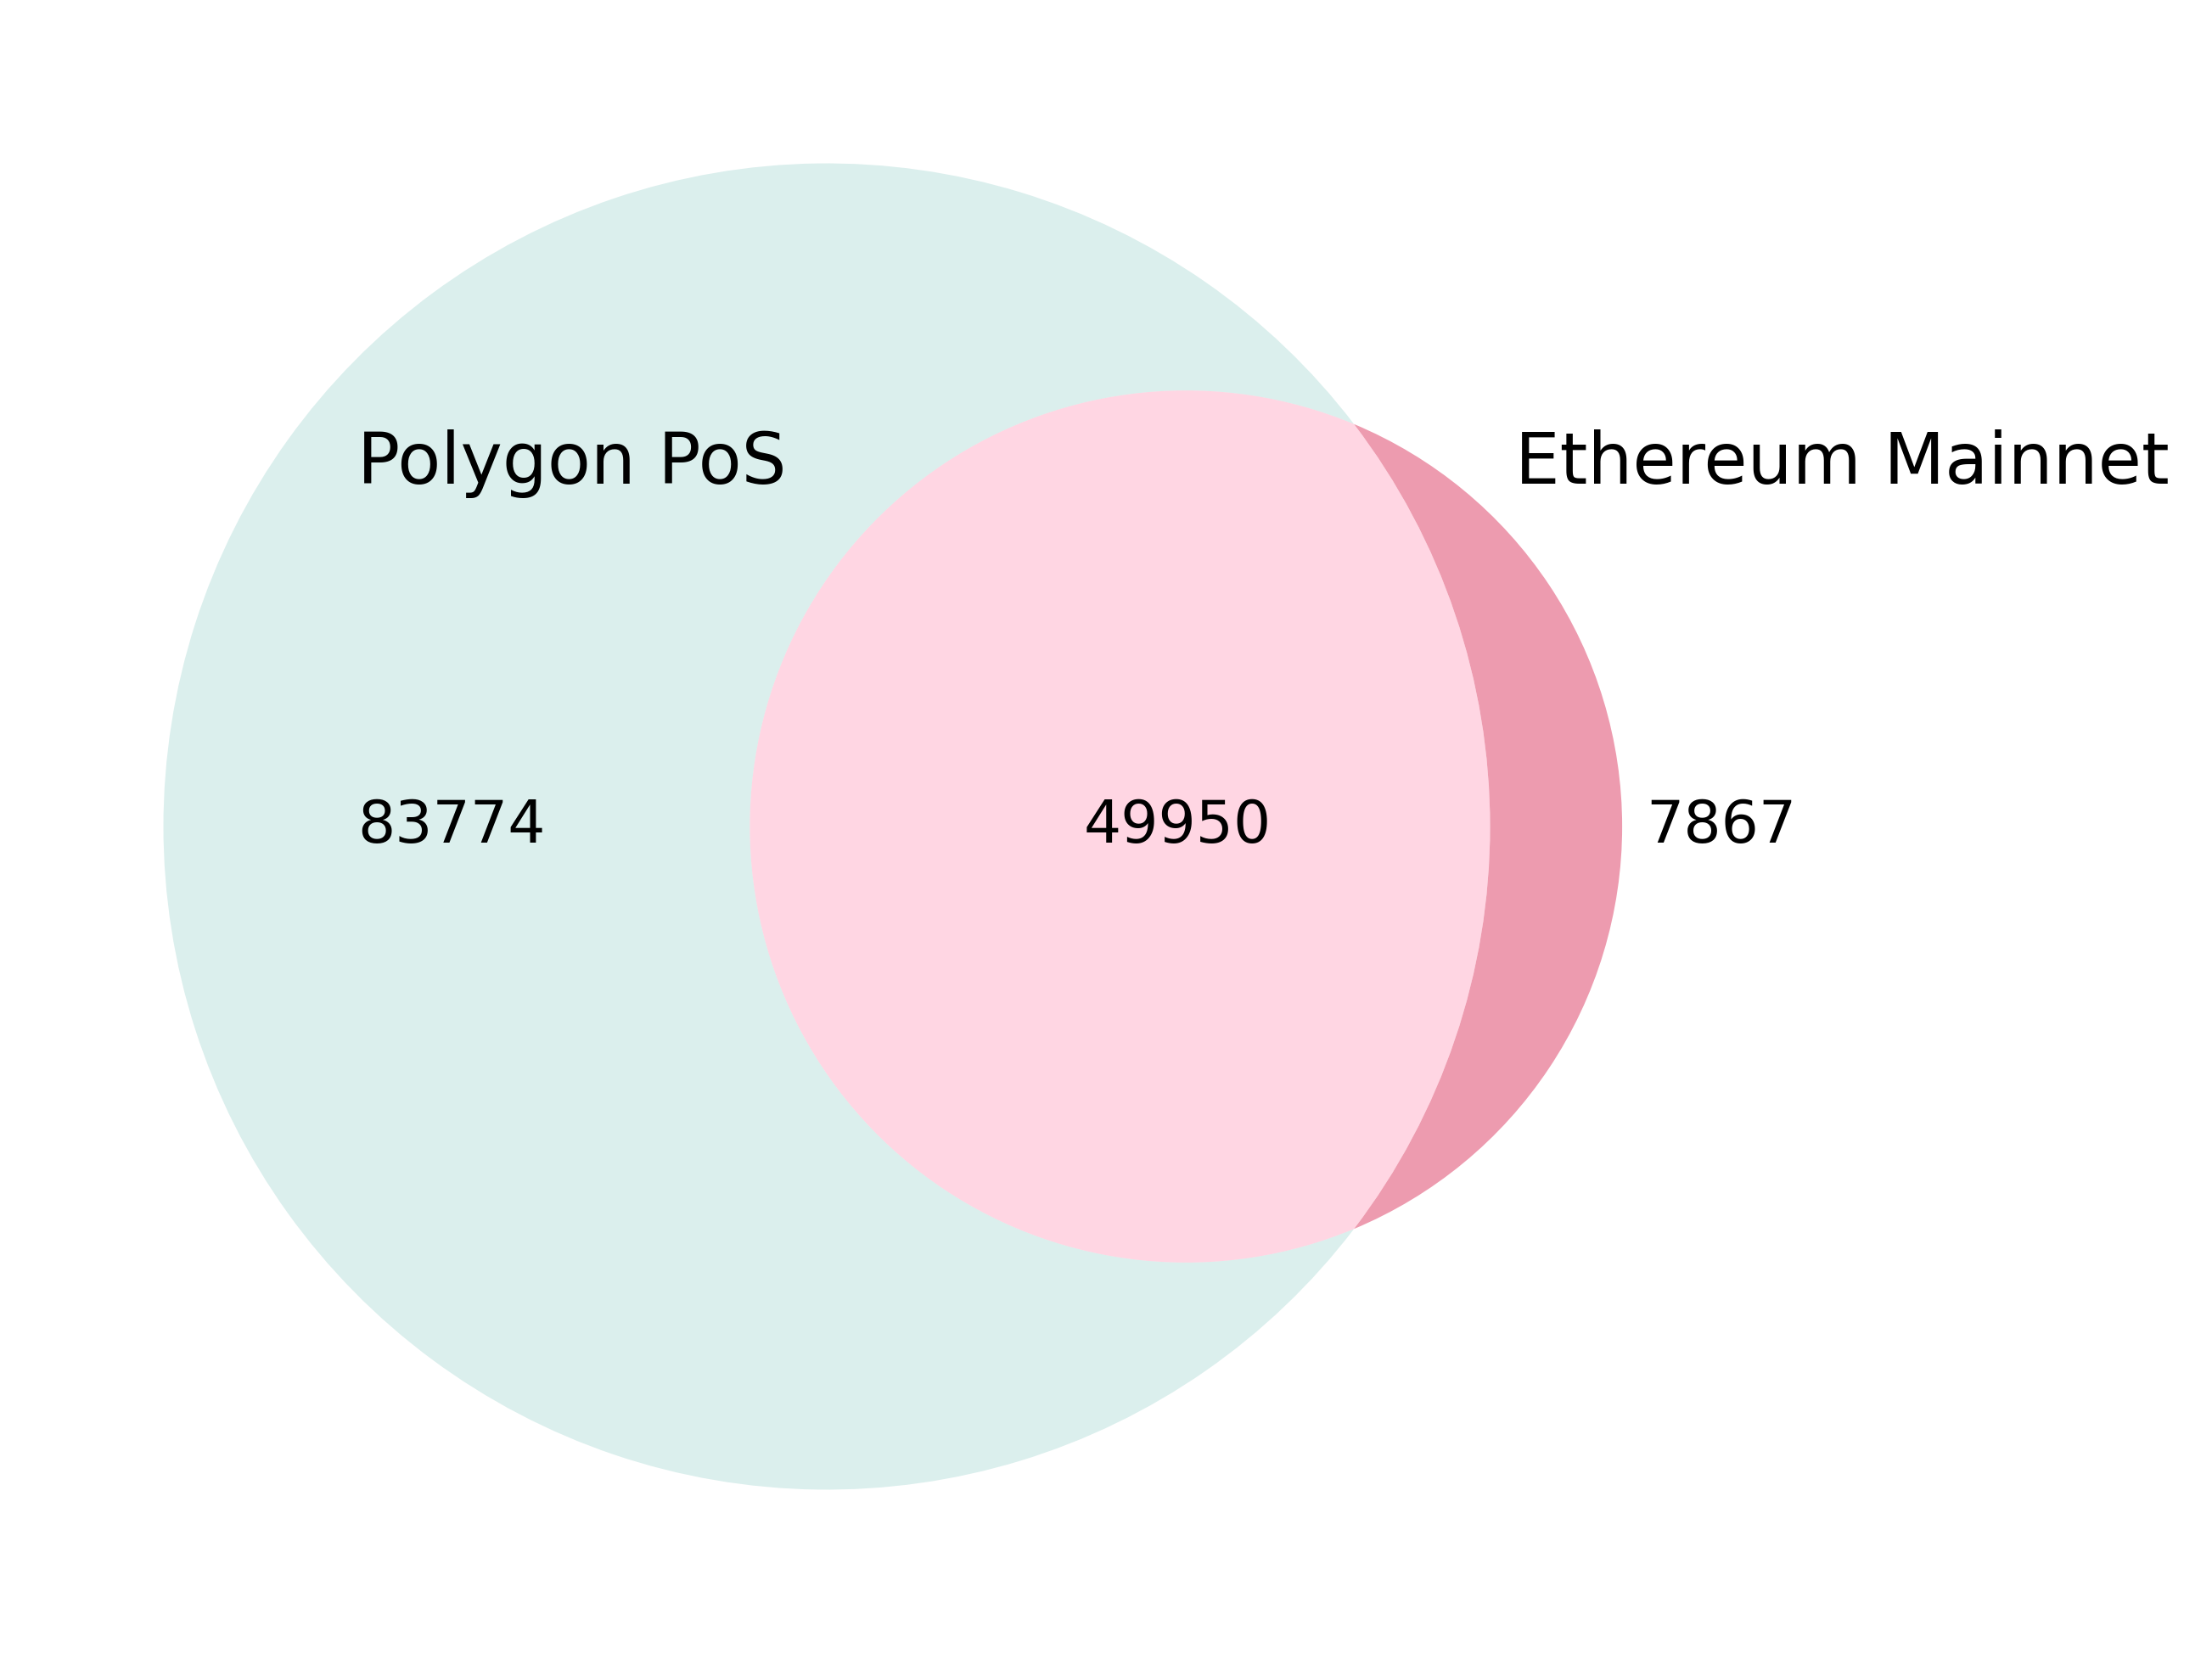
\includegraphics[width=0.6\textwidth]{./figures/venn_diagram.png}
	\caption{Network Specific Address Subsets}
	\label{fig:Venn}
\end{figure} 

\subsection{Transactions and Token Transfer Events}
The address subsets were used to collect transaction and token transfer event data from Ethereum and Polygon. Ethereum or Polygon data can be accessed directly through a node or an application programming interface (API) provider like Infura or Etherscan. The absence of account indexing in Ethereum or Polygon poses a challenge for retrieving all past transactions and token transfers of a specific address, as it requires scanning through all blocks and token transfer events emitted by designated token contracts. Fortunately, Etherscan offers an API Endpoint for ''Accounts'' that facilitates the retrieval of transactions and token transfer events for a given address. By using our network-specific address subsets, I was able to significantly decrease the number of required API calls. 
I gathered all transactions and token transfers up until block number \texttt{17,670,000} on Ethereum (July 11, 2023) and \texttt{44,990,000} on Polygon (July 12, 2023). In total, I collected over 30 million %30,689,978
token transfer events and more than 16 million %16,092,531
 normal transactions. While the amount of transactions is similar between the two networks, Polygon has roughly three times more transfer events. \newline The output was stored in separate CSV files and imported into a MongoDB\footnote{\url{https://www.mongodb.com/}} database. The database contains distinct collections for transactions and transfers. For additional information on the data fields of each collection, see Appendix \ref{sec:database}. 

\subsection{Intra-Set Asset Transfers}
\label{sec:intra-set}
I want to employ address clustering heuristics to determine the number of entities represented by the remaining 137,544 addresses. %Or, to phrase it differently, do users interact with Decentraland using multiple EOAs, and can identify addresses that belong to the same user?
\newline
To achieve this, I often only consider transactions or token transfer events where both the ''\texttt{from}'' (sender) and the ''\texttt{to}'' (recipient) address are within the address set. I call this reduced data set \textit{intra-set asset transfers}. Regarding normal transactions, this means that only native asset transfers (also called payments) are kept, as almost all addresses are EOAs. \newline
The intra-set asset transfer data set is mainly used to generate the network graphs (see Section \ref{sec:node}).
When clustering addresses using graph-based approaches, this has the advantage that I do not need to differentiate between EOA and smart contract account later on. Furthermore, it allows us to observe and visualize the asset flows between users. In total, there are 974,478 intra-set token transfers and 210,548 intra-set native asset transfers.  %101,621 Matic, 108,927 Ether

\subsection{ENS Address Pairs}
\label{sec:ens}
Similarly to \cite{Beres2020}, I use Ethereum Name Service (ENS) identifiers as ground truth information to evaluate clustering methods.\newline
\textit{ENS} is a naming system that relies on the Ethereum smart contracts. Its main purpose is to map human-readable names, such as \texttt{`alice.eth`}, to machine-readable identifiers, mostly Ethereum addresses. The architecture of ENS comprises two main components: the registry and resolvers. \newline
The \textit{ENS registry} consists of a single smart contract\footnote{The registry contract is ERC-721 compliant, which means that .eth registrations can be transferred in the same way as other NFTs.} that maintains a list of all domains and subdomains, recording the ''owner'' and ''resolver'' for each. The registry allows the owner of a domain to make changes to that data. 
\textit{Resolvers} are responsible for translating names into addresses. Any contract that adheres to the relevant standards may act as a resolver. The process of resolving a name involves two steps: \textit{First}, the registry must be queried to find out which resolver is responsible for the name, and \textit{second}, that resolver must be asked for the response to the query. \citep{ENSdocs} \newline
In addition to regular resolution from name to address, ENS also supports ''reverse resolution'', allowing for a mapping from address back to a name or other metadata. Reverse resolution is accomplished via the %special
 domain \texttt{`addr.reverse`}% and the resolver function \texttt{name()}.
. This domain is owned by a special purpose registrar contract that allocates subdomains to the owner of the matching address - for instance, the address \texttt{`0x1234\dots`} may claim the name \texttt{`1234\dots.addr.reverse`}, and configure a resolver and records on it. The resolver in turn supports the \texttt{name()} function, which returns the ENS domain associated with that address.\newline
 Reverse resolution %(without a library)
 follows the same pattern as forward resolution: Get the resolver for \texttt{`1234....addr.reverse'} (where \texttt{`1234...`} is the address you want to reverse-resolve), and call the \texttt{name()} function on that resolver. However, ENS does not enforce the accuracy of reverse records. This means \texttt{`1234....addr.reverse`} may falsely claim that the name associated to their address is \texttt{`alice.eth`}. 
 
Figure \ref{fig:ENS} illustrates the mechanism that allowed us to generate ground truth pairs in a simplified way: Initially, the domain name \texttt{`foo.eth`} resolves to address \texttt{`0xABC...`}. The owner has also set a reverse resolution for this address, indicated by the the edge from the address to the domain name. Next, the owner decides to change the resolved address to \texttt{`0xDEF...`}, again setting a reverse record.  As a domain can only point to one address at the time, the previous mapping from \texttt{`foo.eth`} to the old address is deleted. However, \texttt{`ABC....addr.reverse`} still points to \texttt{`foo.eth`} and querying the name corresponding to \texttt{`0xABC...`} and \texttt{`0xDEF...`}, will return \texttt{`foo.eth`}.
If this special case occurs, I assume that both addresses belong to the same entity.

\begin{figure*}[h!]
	\begin{center}
		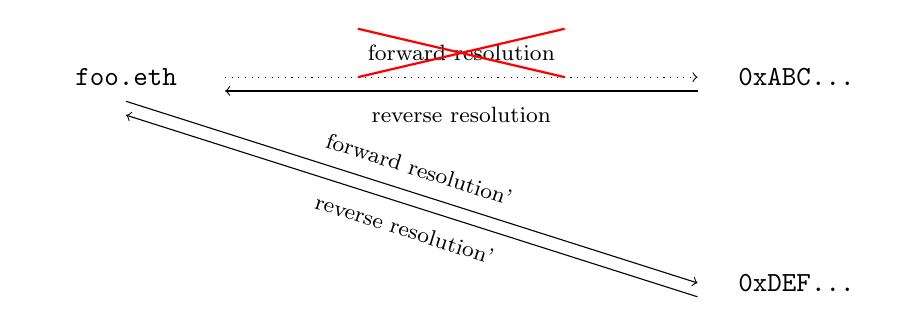
\begin{tikzpicture}[
    every node/.style={minimum width=2.5cm, minimum height=0.6cm, align=center},
    every path/.style={->},
    node distance=2cm and 6cm]

		\node (A) {\texttt{foo.eth}};
		\node[right=of A] (B) {\texttt{0xABC...}};
		\node[below=of B] (C) {\texttt{0xDEF...}};
		
		\draw[dotted] (A) -- (B) node[midway, above, name=pathAB] {\footnotesize{forward resolution}};
		\draw ([yshift=-5pt]B.west) -- ([yshift=-5pt]A.east) node[midway, below] {\footnotesize{reverse resolution}};
		\draw (A.south) -- (C.west) node[midway, sloped, above] {\footnotesize{forward resolution'}};
		\draw ([yshift=-5pt]C.west) -- ([yshift=-5pt]A.south) node[midway, sloped, below] {\footnotesize{reverse resolution'}}; 	
		
		% Adding a cross over "forward resolution"
        \draw[red, thick, -] (pathAB.south west) -- (pathAB.north east);
        \draw[red, thick, -] (pathAB.south east) -- (pathAB.north west);
							
		\end{tikzpicture}
		\caption{Simplified Schematic Representation of an ENS Record Change to Another Address}
		\label{fig:ENS}
	\end{center}
\end{figure*}

I applied the following methodology to find ground truth pairs: \textit{First}, I gathered all addresses that interacted with ENS to reduce the amount of name look-ups. \textit{Second}, I iterated over all addresses and checked if they reverse-resolved to an ENS domain\footnote{This was done via the ENS module within web3.py \url{https://web3py.readthedocs.io/en/stable/ens_overview.html}, which provides an interface to look up domains and addresses.}. If so, I logged the ENS domain and address in a CSV file. \textit{Third}, using our new list, I identified if two addresses referenced the same ENS domain. If matched, I recorded both addresses alongside the ENS domain. \newline
From this, I identified 11,440 reverse records and 40 pairs of addresses pointing to the same ENS name, which I utilized as our ground truth to evaluate various clustering heuristics. Although this sample is relatively small, it allows us to assess and draw conclusions about the effectiveness of the methods.

%From the web3.py documentation \url{https://web3py.readthedocs.io/en/stable/ens_overview.html }
%The ens module is included with web3.py. It provides an interface to look up domains and addresses, add resolver records, or get and set metadata.
%Anyone who owns a domain at any level may configure subdomains - for themselves or others - as desired. For instance, if Alice owns 'alice.eth', she can create 'pay.alice.eth' and configure it as she wishes.

%%%%%%%%%%%%%%%%%%%%%%%%%%%%%
%%% Clustering Heuristics %%%
%%%%%%%%%%%%%%%%%%%%%%%%%%%%%

\section{Clustering Heuristics}
In this section, I present an overview of clustering heuristics in the context of account-based blockchains and on-chain data. I will provide a detailed explanation of the mechanics and rationale behind the heuristic and assess its applicability to our case. 
In Section 5, I will implement and evaluate the heuristics I determine to be suitable for our objectives.

\subsection{Self-Authorization} 
	All three token standards require functions to allow another address to transfer tokens on behalf of the actual owner. For the ERC-20 standard, this is achieved through the \texttt{`approve`} function, accepting the spender's address and the token amount as parameters\footnote{\texttt{approve(address spender, uint256 amount)}}. The ERC-721 has two functions dedicated to approvals: One for authorizing the transfer of a specific NFT\footnote{\texttt{approve(address to, uint256 tokenId)}} and one to permit transferring all of the owner's NFTs within the collection\footnote{\texttt{setApprovalForAll(address operator, bool approved)}}. The latter function also appears in the ERC-1155 standard. The approval functionality of these tokens is primarily used in connection with smart contracts (e.g., Decentralized Exchanges or NFT Marketplaces), but can also be applied for regular EOAs. \newline
The \textit{self authorization} heuristic, proposed by \cite{FV:17}, suggests that users might authorize another address they own, possibly for risk distribution across several addresses or for testing purposes. Since all the addresses' transactions are available in our data set, I can easily employ this heuristic.

\subsection{Deposit Address Reuse}
The concept of deposit address reuse was first introduced and systematically utilized by \cite{FV:17} and subsequently adoped by \cite{wu2022tutela}. This heuristic relies on the prevalent practice of crypto exchanges generating unique deposit addresses for each user. These addresses then forward the funds to an exchange's main address. It is highly likely that multiple addresses sending funds to the same deposit address are controlled by the same entity. The key challenge of this approach lies in identifying these deposit addresses, which could either be EOAs or smart contracts. \citep{FV:17}\newline
Deposit addresses share the characteristic that they forward the received funds to a major exchange account. Two parameters are essential for deposit address detection: the discrepancy between the amount received and forwarded, as the exchange must pay for gas fees, and the time lag between receiving and forwarding funds.
However, our data set only includes the transactions or token transfers associated with the addresses. The transactions between deposit and exchange address are absent. Consequently, this clustering heuristic is not applicable and would require significantly more effort for gathering the required data.

\subsection{Airdrop Multi Participation}
Airdrops are popular token distribution mechanisms, and recipients are mostly chosen based on past protocol activity. Probably the most well known example is Uniswap's UNI airdrop, where each address that ever called the Uniswap V1 or V2 contracts until a specified cutoff date received a fixed amount of 400 UNI tokens\footnote{\url{https://blog.uniswap.org/uni}}. Especially in the early days of airdrops, these distribution mechanisms were not Sybil-resistant, leading to people creating multiple addresses in anticipation of an airdrop. However, \cite{FV:17} argues that managing the tokens on all of these addresses is impractical, which is why they are often aggregated into one address. He found around 500 same-source, fixed amount token distribution events with at least 1,000 recipients while also taking into account the block difference between the individual aidrop token transfers. He defined multi-participation when two airdrop recipients forward their tokens to a single address. Since the whole view of the airdrop distribution events is not available, I am not able to identify them within our data. One possible approach would include manual selection of known airdrops. However, this process takes a long time and is not guaranteed to cluster many addresses, since more recent airdrop events were mostly carried out with some kind of Sybil-resistance. Nevertheless, to test this approach I searched for addresses that forwarded the UNI airdrop to another address. I found eight such transfers, but none involved two addresses sending funds to a third address.

\subsection{Graph Representation Learning}
\label{sec:node}
According to \cite{Beres2020}, \textit{node embedding} algorithms form a class of graph representation learning\footnote{Sometimes also referred to as ''network representation learning''} methods that map graph nodes to vectors in a low-dimensional vector space. These methods aim to represent vertices with similar neighborhood structure by vectors that are close in the vector space. \newline
\cite{Beres2020} first introduced this approach on an Ethereum transaction graph for the purpose of entity identification to pair Ethereum addresses associated with Tornado cash deposits and withdrawals. Building on this, \cite{wu2022tutela} refined and expanded one particular node embedding algorithm to deanonymize Ethereum users at scale. \newline
The foundation for these node-embedding algorithms is an undirected graph where nodes are composed of distinct addresses, and an edge is placed between two nodes if there is a transaction between them. \newline
To construct the network graph, I use the intra-set asset transfers described in section \ref{sec:intra-set}. Our approach differs from the methodologies adopted by \cite{Beres2020} and \cite{wu2022tutela}. On the one hand, \cite{Beres2020} collected all transactions and token transfer events of their address set but did not refine this data to only include intra-set asset transfers. On the other hand, \cite{wu2022tutela} do not operate on a specific address set but use all Ethereum transactions to build the network graph, ignoring token transfer events. After comparing these two methodologies with ours, I determined that intra-set asset transfers were the most effective for clustering a predefined set of addresses. %using node-embedding methods.
\newline
Using the network graph, node embedding algorithms seek to learn a function that projects a node to a $d$-dimensional vector representation (also called feature vector). This is a way of simplifying the graph information by associating each node with a point in the Euclidean space. Various node embedding algorithms have been developed and applied to different domains. \citep{rozemberczki2020difftovec} \newline
The intuition behind node embeddings is that addresses interacting with the same set of addresses within the network graph should be close in Euclidean distance. \cite{Beres2020} cites two main reasons for this. \textit{First}, users with multiple accounts often interact with the same addresses or services from most of them. \textit{Second}, when users move funds between their personal addresses, they may unintentionally reveal their address clusters. \newline
\cite{karateclub} provide a variety of node embedding algorithms as a Python library\footnote{\url{https://github.com/benedekrozemberczki/karateclub}}. They categorize the methods into neighborhood (proximity) preserving and structural. \newline
I focus on the three methods that performed best in \cite{Beres2020} experiments: \textit{Diff2Vec} \citep{rozemberczki2020difftovec}, \textit{Role2Vec} \citep{ahmed2018roletovec}, and \textit{DeepWalk} \citep{perozzi2014}. Diff2Vec and DeepWalk are neighborhood-preserving methods, while Role2Vec is a structural node embedding method. Although all methods utilize random walks to capture graph information, their approaches to leveraging these random walks for constructing Euclidean feature vectors differ. A detailed explanation of each algorithm is beyond the scope of this work. The interested reader may consult the original publications. For a concise overview of Diff2Vec, please refer to \cite{wu2022tutela}. \newline
With our intra-set asset transfer data (\ref{sec:intra-set}) and ENS address pairs (\ref{sec:ens}), I was able to apply and evaluate the node embedding methods described above. To use the library described by \cite{karateclub}, certain preprocessing steps for the network graph are required. Transactions must be treated as undirected edges, loops (self-transactions) and multi-edges must be removed. Moreover, nodes outside the largest connected component are excluded. The resulting network graph includes 51,566 nodes and 249,302 edges. \newline
It is worth noting that unlike \cite{wu2022tutela}, I decided not to include edge weights. For instance, if Alice sent Bob Ether three times and Bob sent Alice Ether two times, the edge weight would correspond to five. This choice facilitated the application of \cite{rozemberczki2020difftovec}'s library and eliminated the need to develop a custom method. Based on our network graph, I generate 128-dimensional feature vectors for each address and method. \newline
Given a node embedding, I can search for the closest $k$ vectors to any given vector. As in \cite{wu2022tutela}, I accomplish this using FAISS (Facebook AI Similarity Search), developed by \cite{johnson2019faiss}, which always returns a list of $k$ nodes, ranked by their Euclidean distance to the given node\footnote{I set $k = 51566$, the total number of nodes in the network graph}. \newline
For evaluation of the three node embedding algorithms, I use our ENS address pairs as ground truth. I run each node embedding method ten times and report the average rank of the target address. For comparison, I compute the mean, median, and standard deviation of the average rank for each method.

\subsection{Time-of-Day Transaction Activity and Gas Price Selection}
Apart from applying node embedding methods to Ethereum transaction graphs, \cite{Beres2020} suggest employing clustering heuristics based on time-of-day transaction activity and gas price selection patterns. \newline
\textit{Time-of-day transaction activity} considers all transaction timestamps initiated by a particular address. These UNIX timestamps are transformed into hour-of-the-day-based values. The authors argue that account owners may expose daily activity patterns and represent addresses by a vector including the mean, median, and standard deviation, as well as an activity histogram divided into four to six-hour bins \citep{Beres2020}.  Figure \ref{fig:ToD} illustrates the time-of-day activity histogram and kernel density estimation (KDE) for a selected ENS address pair, divided into two-hour intervals.\newline
Additionally, the \textit{gas price distribution} heuristic leverages the possibility of users revealing patterns when choosing their gas price. Prior to EIP-1559\footnote{\url{https://eips.ethereum.org/EIPS/eip-1559}}, users could set the gas price manually. In practice, most wallet user interfaces offered three levels of gas prices: slow, average, and fast. Selecting the fast option would ensure almost immediate inclusion in the blockchain. To account for changes in Ethereum traffic volume, the gas price is normalized by the daily network average. The combination of gas price levels users select forms their personal gas price profile. An account is represented by a vector including the mean, median, and standard deviation and a normalized gas price histogram divided into 50 bins, which they determined optimal for clustering performance. \citep{Beres2020} \newline
Both methods will not be employed due to their significantly poorer stand-alone performance compared to node embeddings. Nevertheless, I test a two-step approach: In the first step, I implement Diff2Vec to find the ten nearest neighbors. In the second step, I order the remaining addresses by their Euclidean distance derived from the time-of-day and/or gas price feature vectors. I analyze the impact of this two-step approach on the average rank of a target address.

\begin{figure}[h!]
	\centering
	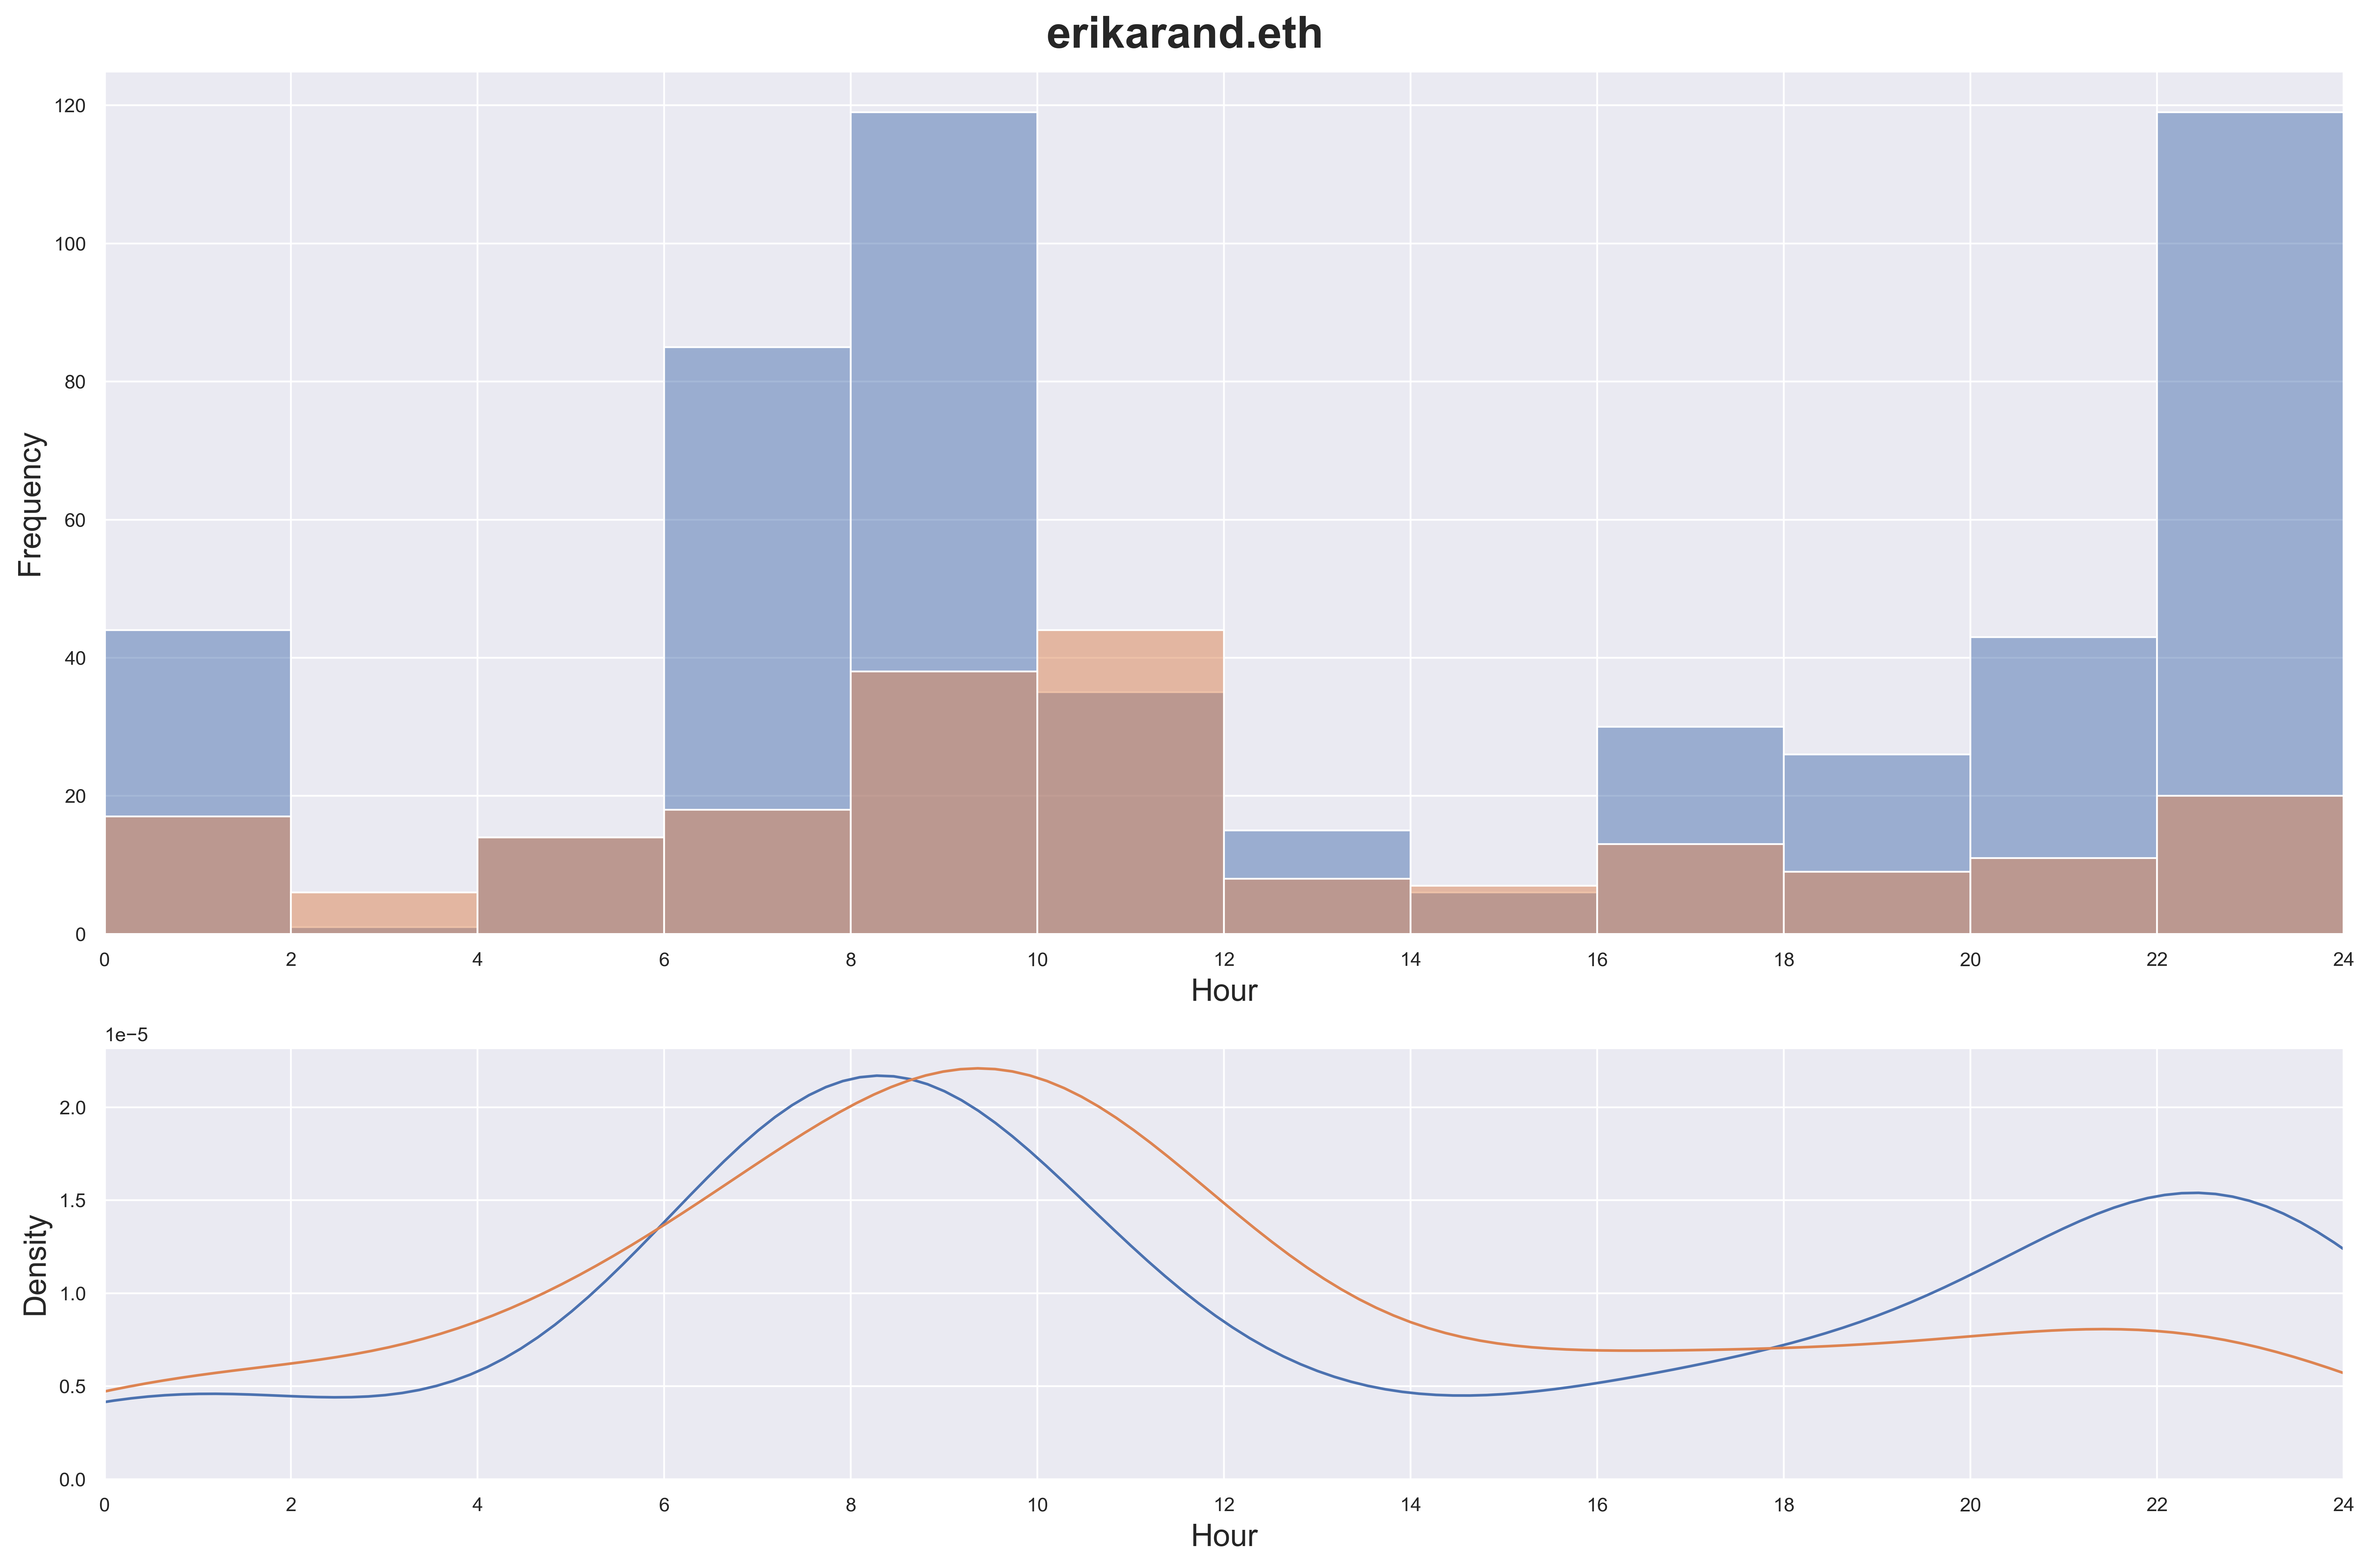
\includegraphics[width=0.9\textwidth]{./figures/time-of-day-activity.png}
	\caption{Time-of-Day Activity Histogram and KDE for a Selected ENS Address Pair, Own Illustration Based on \cite{Beres2020}}
	\label{fig:ToD}
\end{figure} 

\subsection{Tornado Cash Heuristics}
\cite{wu2022tutela} propose five heuristics targeted at Tornado cash, highlighting that careless user behavior can still reveal identity despite using a mixer. The heuristics they identified are as follows: \newline
\textit{Address match} refers to instances where individuals use the same address to deposit and withdraw from the Tornado pool. \textit{Unique gas price} involves users selecting a distinct gas price for their deposit and withdrawal transactions (prior to EIP-1559). \textit{Linked ETH addresses} examines whether a deposit address interacts with a withdrawal address outside Tornado Cash. \textit{Multiple denomination} assesses an address' transaction history; two addresses with matching deposit and withdrawal portfolios are considered a pair. \textit{Torn minting} identifies a specific user behavior when withdrawing so-called Anonymity points, an incentive scheme reward for increasing the anonymity set when depositing assets into Tornado cash.\newline
I identified 84 transactions tied to Tornado cash pools, including 72 deposits, ten withdrawals, and two transactions where an address sent 0.1 Ether to the corresponding pool without invoking the deposit function.  Despite applying all clustering heuristics except Torn minting, no clusters were found.

\subsection{LAND Transfers}
In addition to the existing clustering heuristics, I propose our heuristic based on transfers of high-value NFTs such as LAND. I argue that, given the high value of Decentraland's land parcels, there is a strong likelihood that addresses are controlled by the same entity when LAND is transferred without any compensation. Users might perform such transfers to rearrange their LAND holdings, e.g., by upgrading to a more secure wallet. \newline
The primary challenge of this approach is to detect LAND transfers without any compensation. To accomplish this, I identify token or native asset transfers within the same transaction as a LAND transfer. Upon manually examining various implementations of LAND trades on the most popular NFT marketplace contracts, I noticed a recurring pattern: the user address appears in both the \texttt{''from''} and \texttt{''to''} fields if a trade occurs. Figure \ref{fig:LAND_example} illustrates an example of this pattern. 
In the case of pure LAND transfers, the sending and receiving addresses are the same for all transfers within a transaction. However, this approach does not consider other LAND trading schemes, including off-chain compensation or non-atomic (within multiple transactions) trade settlement.

\begin{figure}[h!]
	\centering
	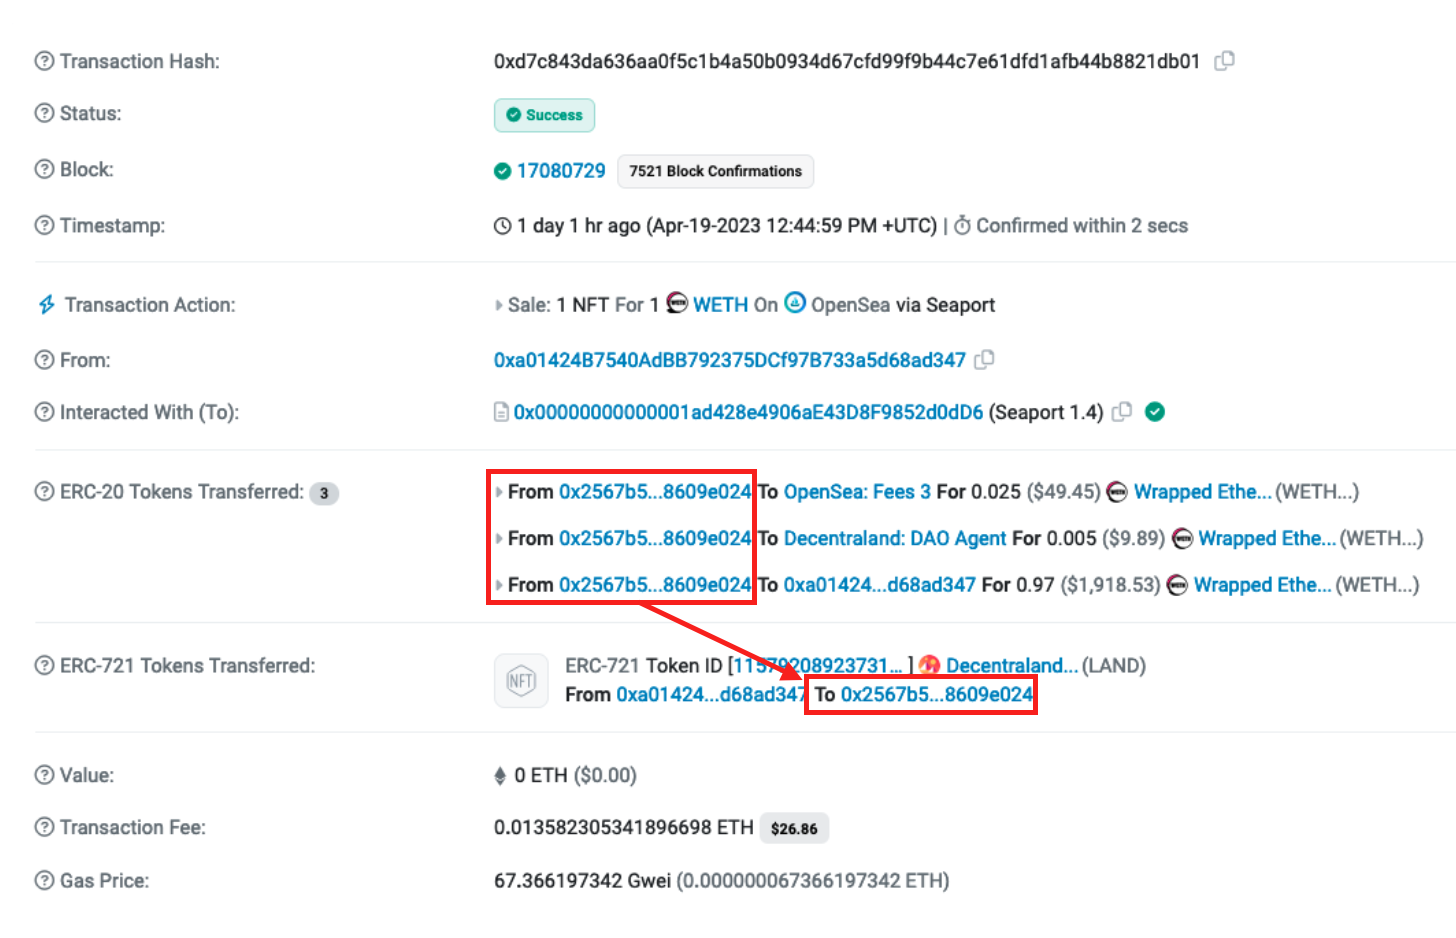
\includegraphics[width=\textwidth]{./figures/etherscan-opensea.png}
	\caption{Example of LAND Trade on Opensea, Source: \href{https://etherscan.io/tx/0x2c2a70114e9080596bf5da6ad9c9b9f6d7e4c85a9d3b06e992f7248f9457a2ec}{Etherscan}}
	\label{fig:LAND_example}
\end{figure}

%%%%%%%%%%%%%%%%%%%%%
%%% Data Analysis %%%
%%%%%%%%%%%%%%%%%%%%%

\section{Data Analysis}
This section analyzes clustering heuristics applicable to our address set using the collected data. These include self-authorization, node embedding, and our proposed approach involving LAND transfers.

\subsection{Self-Authorization}
I analyze the addresses' transaction data to find self-authorizations, focusing on the transaction's ''calldata''. The first four bytes of the calldata represent the function selector, which unambiguously specifies the smart contract function the transaction originator wants to invoke. \newline
\textit{First}, I identify all transactions that begin with a function signature related to the approval functions corresponding to ERC-20, ERC-721, and ERC-1155 token standards. \textit{Second}, I extract the approved (spender) address, which is always located at the same position within the calldata due to token standardization. I then record the spender address in a new field within our data frame. \textit{Third}, I implement two filters on the approval transactions. The first filter checks if the spender address is part of our address set, and the second ensures that the spender address is different from the address initiating the transaction, which may occur due to a user interface bug or testing transactions. \textit{Fourth}, I group the remaining approvals by the initiating address and form the clusters.

I identified 16 clusters across 126 self-authorizing transactions, comprising 115 distinct addresses. After manual inspection, I excluded a cluster containing 80 addresses with all approvals issued by the same address for the same token contract. The token contract represents a collection of wearable NFTs on Polygon called ''Renaissance King by René Mäkelä'' and may use an uncommon or potentially even faulty token minting scheme. Ultimately, I discovered 35 addresses associated with 15 distinct entities.

\subsection{Node Embeddings}
Our analysis of node embedding methods starts with a network graph built from intra-set asset transfers. I treat addresses as nodes and add undirected edges between them if they interacted with each other. \newline
To use the Python library developed by \cite{karateclub}, I remove multi-edges and loops (i.e., transfers with the same sender and recipient address) and only consider nodes within the largest connected component. The resulting network graph includes 51,566 nodes and 249,302 edges. As previously stated, I utilize the Diff2Vec, Role2Vec, and DeepWalk methods from the library. \newline
Subsequently, I ran ten independent experiments for each method. Our choice of input parameters is identical to \cite{Beres2020}. Each experiment returns a node embedding in a matrix with 51,566 rows corresponding to the number of nodes in the graph and 128 columns representing the feature vector dimensions. \newline
For any node within the embedding, I can easily order all other nodes by the Euclidean distance. I achieve this through the FAISS Python library, which is suitable for efficient similarity search and clustering of dense vectors \citep{johnson2019faiss}.\newline 
This feature enables us to search for our ENS ground truth pairs and report their relative rank. The results for each address pair, averaged over ten experiments, are presented in Table \ref{tbl:ENS_Domain_Ranks}. Additionally, I calculated the mean, median, standard deviation, and the rate of the target address appearing within the five or ten nearest neighbors for each method.

All three methods demonstrated remarkable efficacy in locating the target address, which indicates their ability to find multiple addresses controlled by a single entity.
Role2Vec is the most effective method, with the target address, on average, found within the 28 nearest neighbors. In contrast, Diff2Vec and DeepWalk produced slightly higher averages of 46 and 62, respectively. Furthermore, Role2Vec found the target address within the ten nearest neighbors in 24 out of 34 cases (71\%). Diff2Vec is barely less effective than Role2Vec or DeepWalk, although it is still generally successful. \newline
Notably, two address pairs are absent within the network graph and, therefore, display no values. However, they have been included to demonstrate that the intra-set asset transfer approach may not always be applicable to cluster all addresses of a predefined set.

\begin{table}[h!]
\scriptsize
  \centering
  \begin{tabular}{lrrr}
    \hline
	\textbf{User} & \textbf{Diff2Vec} & \textbf{Role2Vec} & \textbf{DeepWalk} \\
	\hline
    1 & 2.5 & 6.2 & 2.7 \\
    2 & 577.3 & 33.3 & 58.8 \\
    3 & 2.8 & 2.5 & 3.3 \\
    4 & 106.8 & 71.1 & 20.1 \\
    5 & - & - & - \\
    6 & 11.1 & 3.0 & 1.4 \\
    7 & 30.7 & 1.0 & 1.0 \\
    8 & 44.3 & 91.2 & 545.4 \\
    9 & 16.3 & 10.4 & 4.1 \\
    10 & 1.0 & 1.0 & 1.0 \\
    11 & 129.1 & 10.0 & 605.4 \\
    12 & - & - & - \\
    13 & 1.0 & 1.0 & 1.8 \\
    14 & 1.9 & 1.0 & 1.0 \\
    15 & 10.4 & 1.0 & 18.2 \\
    16 & 4.0 & 1.0 & 10.3 \\
    17 & 4.2 & 1.5 & 27.2 \\
    18 & 5.7 & 5.6 & 108.5 \\
    19 & 52.3 & 373.8 & 9.0 \\
    20 & 9.0 & 9.0 & 51.8 \\
    21 & 474.2 & 86.7 & 2.4 \\
    22 & 1.7 & 5.0 & 1.0 \\
    23 & 2.7 & 1.0 & 2.3 \\
    24 & 1.3 & 3.4 & 2.4 \\
    25 & 1.0 & 1.0 & 2.2 \\
    26 & 3.7 & 2.0 & 284.0 \\
    27 & 16.9 & 14.4 & 2.2 \\
    28 & 3.6 & 2.6 & 1.7 \\
    29 & 1.5 & 2.0 & 1.6 \\
    30 & 2.7 & 1.0 & 1.1 \\
    31 & 2.0 & 13.6 & 101.2 \\
    32 & 64.8 & 1.1 & 1.6 \\
    33 & 3.0 & 19.3 & 1.7 \\
    34 & 11.0 & 5.6 & 3.4 \\
    35 & 52.1 & 68.9 & 47.3 \\
    36 & 10.3 & 4.0 & 227.0 \\
    \hline
    Mean & 46.038 & 28.073 & 62.084 \\
    Median & 4.2 & 3.4 & 3.3 \\
    Standard Deviation & 120.504 & 68.814 &  139.932\\
    Within 5 nearest & 17 (0.5) & 19 (0.56) & 20 (0.59) \\
    Within 10 nearest & 19 (0.56) & 24 (0.71) & 21 (0.62)\\
    \hline
  \end{tabular}
  \caption{Average Rank of Target Address}
  \label{tbl:ENS_Domain_Ranks}
\end{table}

After evaluating the different node embedding methods, we want to cluster the addresses to assess the number of entities represented by the 51,566 nodes in the network. We use the node embedding generated by Role2Vec. \newline
One approach might involve grouping a node's $k$ nearest neighbors to a cluster and subsequently merging clusters until each node is assigned to exactly one cluster. However, selecting an appropriate $k$ is challenging, and making the case that each address belongs to a cluster of at least $k$ is problematic. \newline
Instead, we choose to build clusters based on Euclidean distance, where all neighbors of a node below a certain threshold are clustered. Afterward, we merge overlapping clusters; for instance, if node A is clustered with nodes B and C, and node C is clustered with nodes A and X, we form a cluster comprising A, B, C, and X. \newline
We explore the sensitivity of clusters to various Euclidean distance threshold values. Figure \ref{fig:threshold_sensitivity} shows the histogram of cluster sizes, and Table \ref{tbl:cluster_table} displays the number of resulting clusters depending on various threshold values. We chose said values after observing the distance between ground truth pairs. For better visibility, we only display clusters below 20 addresses in Figure \ref{fig:threshold_sensitivity}. At thresholds of 0.6, 0.7, and 0.8, we find 23,608, 18,592, and 14,793 clusters, respectively. Regardless of the threshold, the largest cluster has more than 500 addresses. Unsurprisingly, higher thresholds result in fewer single-address clusters and more large-sized clusters. The effect of the threshold is most pronounced for single address clusters while affecting other cluster sizes much less. 

\begin{figure}[h!]
	\centering
	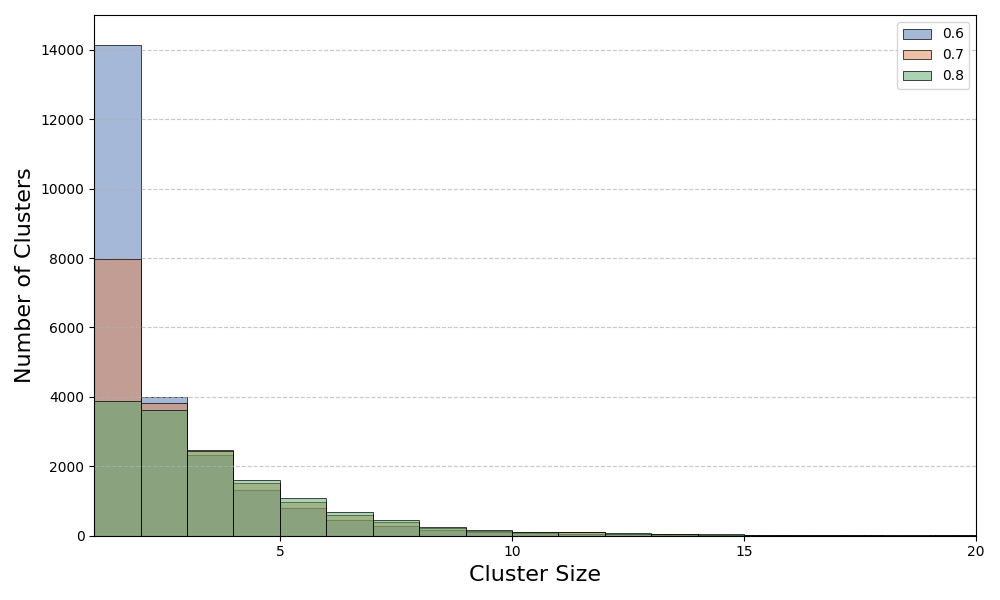
\includegraphics[width=0.9\textwidth]{./figures/cluster_histogram.png}
	\caption{Cluster Size Histogram for Different Distance Thresholds}
	\label{fig:threshold_sensitivity}
\end{figure}


\begin{table}[h!]
\scriptsize
  \centering
  \begin{tabular}{lrrrrrrr}
    \hline
	\textbf{Threshold} & \textbf{0.5} & \textbf{0.55} &\textbf{0.6} & \textbf{0.65} & \textbf{0.7} & \textbf{0.75} & \textbf{0.8} \\
	\hline
Total clusters 			& 29,502 & 26,762 & 23,608 & 21,229 & 18,592 & 16,361 & 14,793 \\
Size of largest cluster & 499 & 	512 & 516 & 	524 & 532 & 535 & 544\\
Clusters of size 50+ 	& 2 & 2 & 3 & 7 & 9  & 13 & 14\\
    \hline
  \end{tabular}
  \caption{Clustering Results for Different Threshold Values}
  \label{tbl:cluster_table}
\end{table}

\subsection{LAND Transfers}
To implement the LAND transfer clustering heuristic, we select all transaction hashes of LAND transfers that occurred between two Decentraland addresses. Next, we gather all token and native asset transfers associated with the selected transaction hashes. We group the data by transaction hash and examine each transfer's sender (\texttt{from}) and recipient (\texttt{to}) address. If the same address appears as the sender and recipient, we mark the transaction as a purchase. Finally, we exclude purchases and build clusters for addresses that sent each other LAND without compensation. \newline
A total of 2159 intra-set LAND transfers were recorded, of those, 677 (X \%) were without compensation. We were able to group the 413 unique addresses from these uncompensated transfers into 161 distinct clusters. 
Notably, the majority of clusters consist of two or three addresses. However, one cluster counting 71 addresses stands out. \newline 
Figure \ref{fig:LAND_network} visualizes LAND transfers between Decentraland addresses as a token network graph. In this graph, red edges signify non-compensated transfers, whereas blue edges represent LAND transfers made as part of a trade/purchase. Notably, the 71-address cluster previously mentioned is visible on the top-right of the largest connected component. \newline
A few key observations can be drawn from this network graph. In line with our expectations, most LAND transfers involve some form of compensation. Moreover, certain nodes play a central role in LAND trading activity, indicated by their high connectivity within the network. Lastly, a recurring behavior pattern is observed wherein an individual address purchases LAND and subsequently transfers it to a third address.

%\begin{figure}[h!]
%	\centering
%	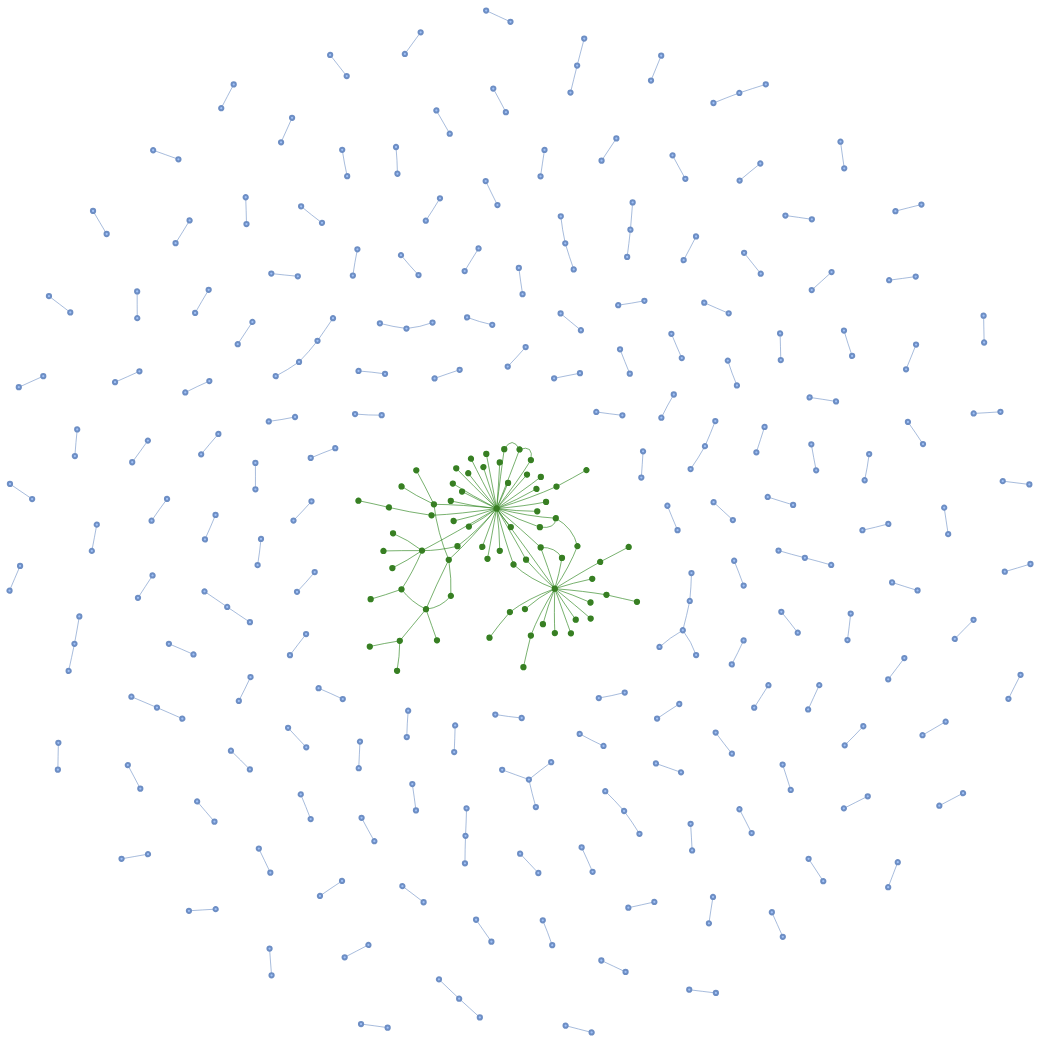
\includegraphics[width=0.5\textwidth]{../figures/land_clusters.png}
%	\caption{LAND Entity Clusters (largest cluster marked in green)}
%	\label{fig:LAND_clusters}
%\end{figure}

\begin{figure}[h!]
	\centering
	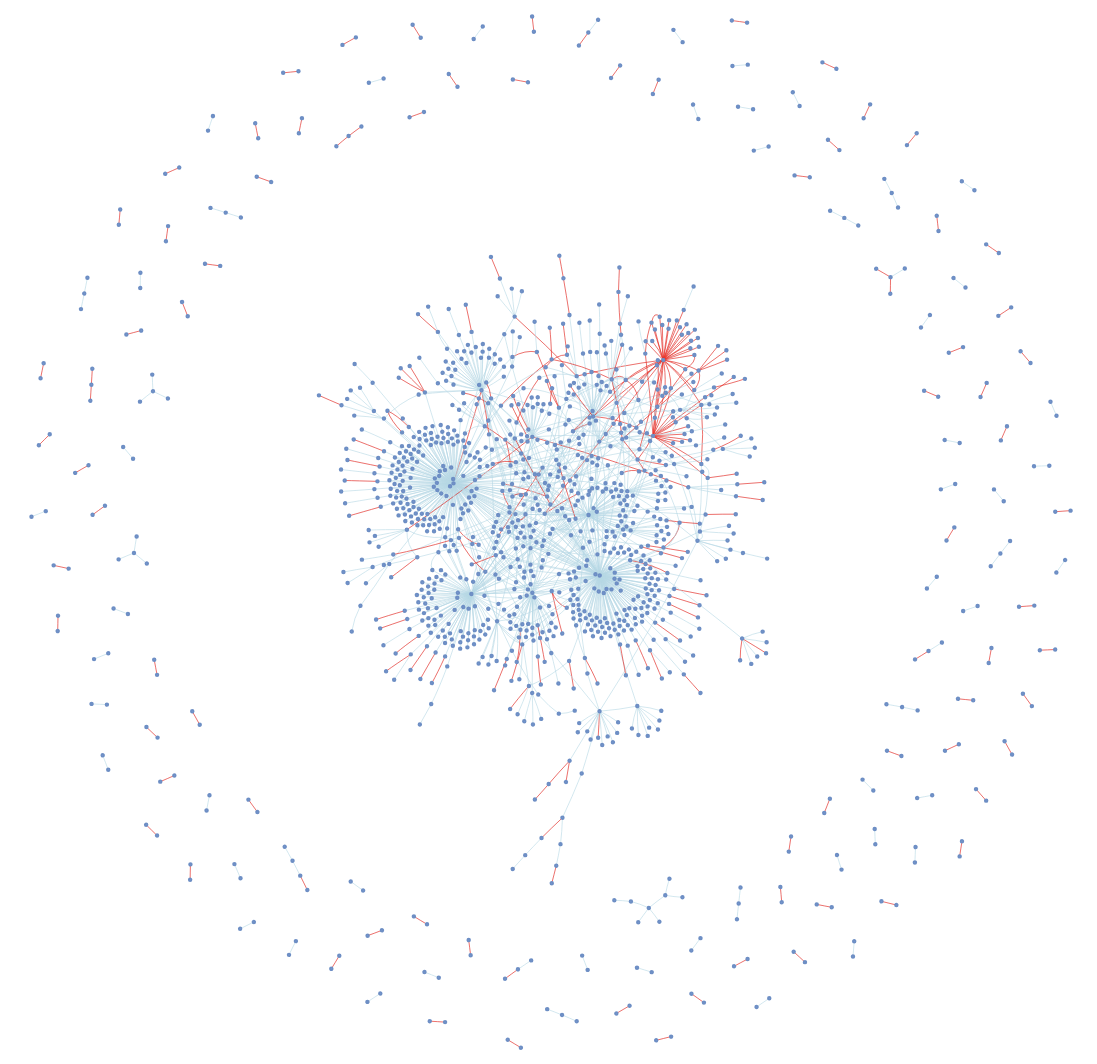
\includegraphics[width=0.9\textwidth]{./figures/land_network.png}
	\caption{LAND Transfer Network of Address Set}
	\label{fig:LAND_network}
\end{figure} 

\subsection{Combining Clustering Results}
To conclude our clustering analysis, we combine the results of self-authorization, learned node embedding, and LAND transfer heuristics. By doing so, we can cluster 51,581 out of 137,544 (37.5\%) addresses representing 29,680 entities. 
For the remaining addresses, we consider each as an individual entity. 
We applied a strict distance threshold of 0.5 for clustering embeddings generated by Role2Vec and excluded the 80-address cluster identified in self-authorization.
Under these assumptions, we estimate 115,643 active users during the time frame studied. Of these, 8,483 entities (7.3\%) interacted with Decentraland through multiple addresses. The largest entity comprises 499 addresses. We plot the distribution of cluster sizes in Figure \ref{fig:barplot_clusters}.

\begin{figure}[h]
	\centering
	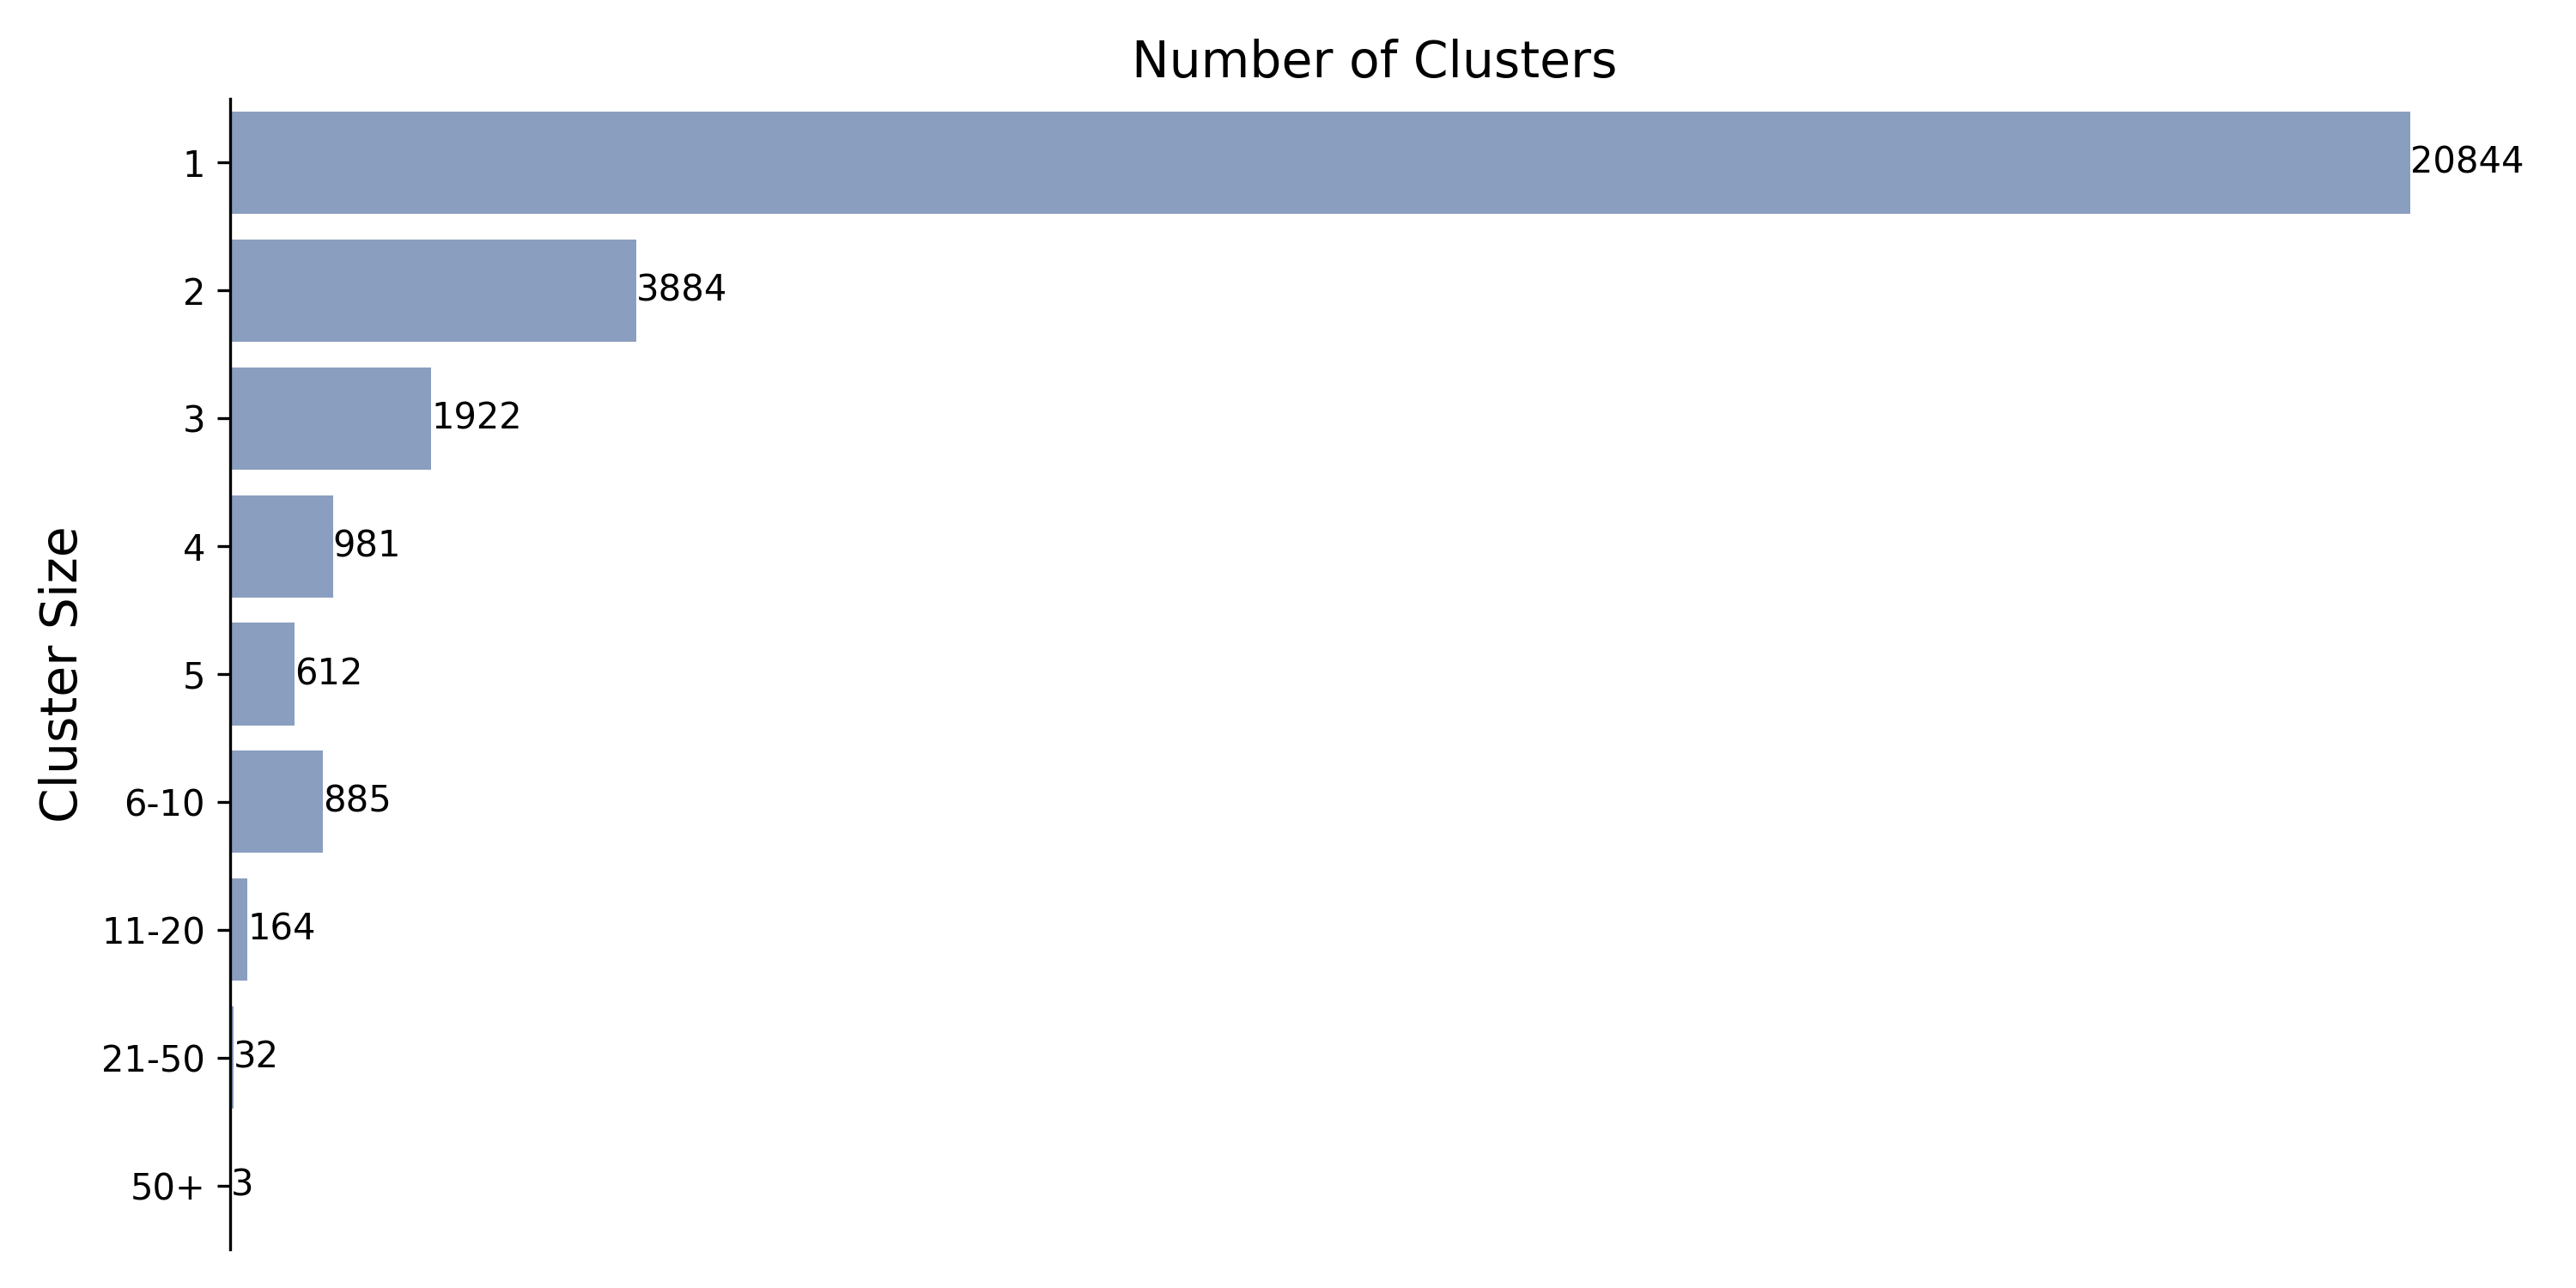
\includegraphics[width=\textwidth]{./figures/cluster-size-distribution.png}
	\caption{Number of Clusters by Cluster Size}
	\label{fig:barplot_clusters}
\end{figure}


%%%%%%%%%%%%%%%%%%
%%% Discussion %%%
%%%%%%%%%%%%%%%%%%

\section{Discussion}
Throughout our analysis, we successfully applied three heuristics to cluster our address set while making use of on-chain data. In the following discussion, we will examine each of the approaches step-by-step.

Implementing the \textit{self-authorization} heuristic is straightforward but results in very few identified address clusters. This is because it requires a highly specific on-chain behavior, which is rarely observed in practice. In particular, approvals are seldom used to authorize another externally owned account one might own. We also encountered a significant number of false positives due to non-standard implementations. We are very confident that the large cluster is not controlled by the same entity, and therefore remove it. After excluding these instances, we identified a total of 15 entities consisting of 35 addresses. This outcome aligns with findings by \cite{FV:17}, who also observed that the heuristic captures only a small proportion of addresses. In his analysis of Ethereum transaction data up to block number \texttt{8,500,000}, he identified 4,599 entities from 7,107 addresses.

Address clustering through \textit{graph representation learning} proved to be the most effective approach in our analysis. Unlike methods that require participation in specific on-chain events, node embedding algorithms examine the entire asset transfer network between addresses, making it broadly applicable. \newline
Our implementation of node embedding methods differs from previous approaches by \cite{Beres2020} and \cite{wu2022tutela}, the main reason being different settings and research questions. We construct the network graph based on asset transfers within our address set and simultaneously analyze Polygon and Ethereum data. \newline
Conversely, \cite{wu2022tutela} aim to cluster addresses without a predefined set, using Ethereum transaction data for network graph construction as a result. \cite{Beres2020} try to match deposit and withdrawal addresses for Tornado Cash, relying on all token transfers and transactions to cluster addresses based on similar on-chain behavior. Since it is not common that Tornado cash withdrawal and deposit addresses interact with each other, the approach chosen by \cite{Beres2020} is better suited for their objectives. \newline
Moreover, we validated our approach and found better results regarding the average rank of ground truth address pairs when building the network graph from intra-set asset transfers compared to using all token transfer events and/or transactions. A possible extension would include incorporating edge weights, similar to \cite{wu2022tutela}; however, we refrained from doing this because we would have needed to implement a custom node embedding algorithm.\newline
We applied three node embedding algorithms that delivered robust results in the experiments by \cite{Beres2020} and assessed their effectiveness in detecting ground truth pairs. Our results indicate that Role2Vec is the best-performing method, locating the ground truth pair within the ten nearest neighbors in 70\% of cases.  This result diverges from the findings of \cite{Beres2020}, who determined Diff2Vec to be the superior method among the three evaluated. \newline
Determining why one approach outperforms another is challenging. DeepWalk and Diff2Vec, both neighborhood-preserving algorithms, mainly capture node proximity. As noted by \cite{ahmed2018roletovec}, this does not necessarily imply similarity, especially when addresses frequently interact without being controlled by the same entity. In contrast, Role2Vec, a structural node embedding method, identifies nodes with similar roles within the network. In our evaluation sample, network position or role may better represent node similarity and structural relatedness. Despite these insights, the differences in results could be specific to the data at hand, given the small sample size, potential evaluation metric flaws, and the overall robust performance of all methods. \newline 
Additionally, our evaluation sample may be biased, as one could argue that users changing the address associated with their ENS domain name while also keeping the reverse records are not primarily concerned with preserving privacy. \newline
We also need to consider that average rank may not be the most appropriate evaluation metric, particularly when a user controls more than two addresses. Suppose a single entity controlling 20 addresses, but only one pair of addresses is detected as ground truth. Even if the algorithm finds all 20 addresses within the nearest neighbors but identifies the ground truth pair as the last one, we will score it lower than another algorithm that finds only one of the twenty addresses within the 10 nearest neighbors. \newline
Creating clusters out of the node embeddings enables us to estimate the number of entities represented by the 51,566 addresses. Our method involves calculating the Euclidean distance between pairs of feature vectors, explicitly using the node embedding matrix generated by Role2Vec. Nodes are clustered if their distance falls below a predetermined threshold, and any overlapping clusters are subsequently merged. \newline 
While our clustering method may not be ideal, it is probably more effective than clustering a fixed number of $k$ neighbors for each node. We observed that the number of clusters and their size is highly sensitive to the chosen distance threshold, making it challenging to assess the accuracy of these clusters. We have provided a sensitivity analysis to illustrate this issue. The distances between the feature vectors tend to be narrow, with significant variation even among various ground truth pairs' distances. Regardless of the threshold value, we were able to locate a cluster of more than 500 addresses. Manual inspection revealed that these addresses show very similar on-chain patterns: They are all exclusively active on Polygon, and most transfers are mints of Decentraland-related NFTs. Further, they transfer some NFTs to address \texttt{''0xE2e2F2240a84A61B7dFF50a86ee10d5FaF7faCa8''}. The transfers to and from this address are shown in Figure \ref{fig:cluster}. Incoming transfers are indicated by green edges, while red edges show outgoing transfers. We hypothesize that the network in question may be operated by a user or even bot that creates multiple distinct addresses and actively engages with Decentraland. It seems likely that this bot may target specific locations or events where NFTs are (automatically) air-dropped to avatars in presence. If the NFTs hold value, the bot may then aggregate them to the main address and sell them on the Decentraland marketplace. This hypothesis could be verified with the Decentraland movement data. \newline
Notably, despite the limited on-chain data available, the node embedding algorithm was able to detect this activity pattern. Bot activity may become a concern for open and permissionless metaverse platforms like Decentraland and an interesting topic for future research. \newline
Finally, we explored potential enhancements to the graph representation learning method, such as incorporating time-of-day-activity and/or gas price selection information into the feature vectors generated by Role2Vec. Unfortunately, these modifications did not lead to any significant improvements. This outcome may be attributed to challenges in implementation, particularly in scaling the values without disturbing the integrity of the dense feature vectors.  
Similarly, a two-step approach for clustering, re-ranking the nearest neighbors of a node according to similarity in time-of-day activity and/or normalized gas price vectors, proved unsuccessful. These ideas remain open for further development of clustering heuristics in the future.

\begin{figure}[h!]
	\centering
	\includegraphics[width=0.8\textwidth]{./figures/network_visualization_0xe2e.png}
	\caption{Token Transfer Graph for \texttt{0xE2e2F$\dots$faCa8}}
	\label{fig:cluster}
\end{figure}

The \textit{LAND transfer} heuristic is targeted at users revealing address clusters by sending high-value assets to other addresses. In this specific case, we use the information that all addresses are related to Decentraland and analyze LAND transfers. However, the approach could be applied to other NFT collections or large asset transfers in general. \newline
The main assumption behind this approach is that users may want to reorganize their accounts from time to time, primarily to increase security guarantees or spread the risk across multiple accounts. As a concrete example, some users may have started with a simple browser-based wallet, but as their assets appreciated in value, they transitioned to a more secure hardware wallet. We detect 161 entities with 413 addresses applying this approach. One cluster with 70 addresses is likely not a single entity. It includes an address that participated in the initial LAND auction and subsequently distributed LAND. This may have happened through off-chain compensation. The advantage of this method is that it is relatively easy to visualize and understand. The disadvantage is that it demands a specific on-chain behavior and is only scalable with significant effort. Additionally, many events that occur off-chain are not detectable in the data, resulting in increased false positives. 

Ultimately, we combined the results for each clustering heuristic mentioned above. Consequently, we managed to cluster 51,518 addresses, corresponding to 29,680 distinct entities. When adding the unclustered addresses, we identified 115,643 active users during the nine months, with 8,483 entities interacting through multiple addresses. \newline
These results, however, are heavily influenced by the assumptions we made. We were conservative by setting a low distance threshold and treating all other addresses as individual entities. Raising the threshold would result in larger clusters and fewer entities. \newline 
The majority of addresses were clustered through graph representation learning methods. Unlike other clustering heuristics, this approach does not rely on specific on-chain behavior patterns or participation in particular events. Our implementation generally captures all addresses that transferred assets within the address set at least once. Nevertheless, some clusters may still go undetected, while others may be overestimated. It is important to note that these methods are heuristic, and testing their efficacy on a large scale is not feasible. \newline
Role2Vec performed best for our small test sample but may not always superior to Diff2Vec or DeepWalk. Incorporating time-of-day and normalized gas into feature vectors or refining clusters using a two-step approach requires further research but could enhance clustering results.

%%%%%%%%%%%%%%%%%%
%%% Conclusion %%%
%%%%%%%%%%%%%%%%%%

\section{Conclusion}
This work aimed to determine how many unique entities correspond to the 473,927 addresses observed in Decentraland from July 16, 2022, to April 23, 2023. \newline
By focusing on Ethereum and Polygon on-chain data, we narrowed the set down to 137,544 addresses. The required data was efficiently sourced by gathering all transactions and token transfers related to the addresses via Etherscan and Polygonscan. Furthermore, with the help of ENS, we found a way to detect address pairs with a very high probability of being controlled by the same user. These address pairs served as our ground truth when evaluating the node embedding algorithms. \newline
We discussed several existing clustering heuristics and evaluated their suitability in our context. Among these heuristics, two were found to be appropriate for clustering a predefined set of addresses with the available data: self-authorization \citep{FV:17} and graph representation learning \citep{Beres2020}. We modified the graph representation learning approach for our research goal. %to align with our research goals, this is the first attempt to utilize intra-set asset transfers in constructing the network graph
To the best of our knowledge, we are the first to employ intra-set asset transfers for constructing the network graph. Moreover, we introduced a novel clustering heuristic that identifies uncompensated transfers of high-value NFTs, particularly LAND. \newline
Due to its general applicability, graph representation learning proved to be the most successful clustering heuristic, while the other two heuristics yielded far fewer address clusters. In our exploration of node embedding algorithms, the Role2Vec algorithm stood out, correctly identifying the ground truth pair within the ten nearest neighbors in 71 percent of the cases. \newline
From the 137,544 addresses transacting on Polygon or Ethereum, we identified an estimated 115,643 active Decentraland users. A subset of 8,483 entities, representing 7.3\%, operated through multiple addresses. Notably, the largest address cluster we observed was an entity with 500 distinct addresses. Based on our analysis, this entity is likely a bot targeting Decentraland NFT airdrops, with intentions to resell them later. \newline
To enhance clustering performance, node embeddings could incorporate time-of-day activity and gas price selection patterns. This approach holds considerable promise for future research in entity identification. \newline
A significant challenge for graph representation learning is the formation of clusters after node embedding. In our study, we relied on an Euclidean distance threshold for this purpose. However, the resulting number and size of clusters are highly sensitive to the precise selection of this threshold. \newline
Notably, our approach is versatile and can be applied to other large predefined address sets. This adaptability is particularly significant given the increasing importance of determining the true number of users in various blockchain applications, especially in areas like Decentralized Finance or on-chain governance. \newline
Although we were able to detect entity clusters, Decentraland still exhibits a lot of natural activity. Its open infrastructure presents vast opportunities for in-depth analysis of the virtual world, as demonstrated in this work. \newline
Address clustering will continue to make further advancements. From a user perspective, it is crucial that privacy-enhancing protocols continue to evolve and gain large-scale adoption. Additionally, education on preserving privacy when transacting on blockchains becomes an increasingly important topic.

%%%%%%%%%%%%%%%%%%%%%%%%
%%% Acknowledgements %%%
%%%%%%%%%%%%%%%%%%%%%%%%
\newpage
\section*{Acknowledgements}
I would like to thank Prof. Dr. Fabian Schär for his advice and support throughout the thesis and the opportunity to delve into this intriguing topic. My gratitude also extends to Mitchell Goldberg for his valuable inputs and discussions. Last but not least, a special thanks to Willy Thürkauf for his proof-reading.

%%%%%%%%%%%%%%%%%%%%%%%%%%%%
%%% Literaturverzeichnis %%%
%%%%%%%%%%%%%%%%%%%%%%%%%%%%

\newpage
\setcounter{page}{1}
\pagenumbering{roman}
\onehalfspacing
\addcontentsline{toc}{section}{References}
\bibliography{mybib}
\bibliographystyle{agsm}

\section{Appendix}

\subsection{Database Schema}
\label{sec:database}


\begin{table}[h!]
  \centering
  \tiny
  \begin{tabular}{ll p{4cm} p{5.5cm}}
    \hline
    \textbf{Collection} & \textbf{Fields} & \textbf{Description} & \textbf{Example} \\ \hline
    Transactions & \texttt{\_id} & Unique identifier & 64b3c65ed2daf924bfdce72b
 \\
    (16.1M rows) & \texttt{hash} & Transaction hash & \seqsplit{0x8d9490e9f0992e68490cfcb126e76290eca3bf668a9ba0295d563e0553ed657d} \\
     & \texttt{timeStamp} & Timestamp in seconds from the UNIX epoch &  1657777314\\
     & \texttt{gasUsed} & Amount of gas used by the transaction &  144176  \\
     & \texttt{gasPrice} & The price of gas the originator is willing to pay &  12449848873 \\
     & \texttt{nonce} & Scalar value equal to the number of transaction sent from an EOA or, in the case of contract accounts, the number of contract-creations made by this account  & 23 \\
     & \texttt{from} & Address initiating the transaction & \seqsplit{0xbf9645420578f66d29145dbe5c4a0ba6a85e7121}  \\
     & \texttt{to} & The destination address (either native asset transfer or function call) & \seqsplit{0x000000000d5a50614bcdf08700fe6ceb1c7dad4b} \\
     & \texttt{value} & The amount of Ether/Matic to send to the destination address & 500 \\
     & \texttt{input} & Calldata & \seqsplit{0x095ea7b30000000000000000000000001111111254fb6c44bac0bed2854e76f90643097dffffffffffffffffffffffffffffffffffffffffffffffffffffffffffffffff} \\
     & \texttt{functionName} & added by Etherscan & approve(address spender, uint256 rawAmount) \\
     & \texttt{chainName} & Chain indicator & Ethereum or Polygon \\
    \hline
    Transfers & \texttt{\_id} & see above & see above\\
    (36.4M rows) & \texttt{hash} & see above & see above \\
     & \texttt{timeStamp} & see above & see above\\
     & \texttt{gasUsed} & see above &  see above\\
     & \texttt{gasPrice} & see above & see above \\
     & \texttt{nonce} &  see above & see above \\
     & \texttt{from} &  Sender address (zero address for mints) & \seqsplit{0x0000000000000000000000000000000000000000} \\
     & \texttt{to} &  Recipient address & \seqsplit{0x000000000d5a50614bcdf08700fe6ceb1c7dad4b} \\
     & \texttt{value} & Amount of tokens transferred in Wei, only for fungible or semi-fungible tokens & 10000000000000000 or NaN (ERC-721) \\
     & \texttt{tokenID} &  Identifier of the NFT or semi-fungible token &  1314 or NaN (ERC20) \\
     & \texttt{contractAddress} & The token contract address &  0xc02aaa39b223fe8d0a0e5c4f27ead9083c756cc2 \\
     & \texttt{tokenName} & The specified token name &  Wrapped Ether\\
     & \texttt{tokenType} & Token standard indicator &  20 or 721 or 1155\\
     & \texttt{chainName} & see above &  see above \\
     & \texttt{isSet} & Indicator if `from` or `to` address are from address set &  from or to \\
     & \texttt{userAddress} & Address of user in set & 0x000000085d9a759bb5c3d459d638739c0f48deb0\\
    \hline
  \end{tabular}
  %\caption{Database/data set Description}
\end{table}
%Distinction: Transaction is a message sent from an externally owned account

\subsection{Github Repository}

The code, figures, and data sets used for this thesis are hosted on Github. The repository is organized into the following directories:

\begin{itemize}
	\item \texttt{python}: Contains all the source code used for data collection, analysis, and visualization.
	\item \texttt{figures}: Contains the figures and plots generated during the analysis. Network Graphs can be viewed as an interactive HTML file.
	\item \texttt{data}: Contains the small data sets used for the analysis.
\end{itemize}

For the complete repository including a documentation of each file and its purpose, please visit the following link:

\texttt{\url{https://github.com/dariothuerkauf/address-clustering}}

%For raw data not available in the repository, please contact the authors directly.
%
%An early version of a generalized address clustering Python module can be found at:
%
%\texttt{\url{https://github.com/dariothuerkauf/intra-set-address-clustering}}
%
%This module fetches the required data from Etherscan and Polygonscan when given a set of addresses as input, applies the Role2Vec algorithm to the resulting intra-set asset transfer data, and then constructs the clusters using a Euclidean Distance threshold. Please note that this module is still under development.


\end{document}
